% =====================================================================
%  PLA DE TREBALL (PT) -- Concurs LE-403/729 (UPC)
%  Version 2 (16/11/2026), built on PT_skeleton.tex. American English, aligned with the
%  HAP (three research lines, HAP numbering of publications [J], [R], [C], [D]).
%  General context on the UPC, the EEBE and the subjects adapted from the PT of
%  J. Calafell and the Professor Agregat project, rewritten in English.
%  Personal data: ONLY name and surname (base 3.5).
%  Before submitting: uncomment \finaltrue to hide the marks.
%  Output file name: Monteiro_Carlos_PT.pdf
% =====================================================================
\documentclass[11pt]{article}
\usepackage{lector}
\usepackage{pgfgantt}
\usepackage{needspace}
\usetikzlibrary{arrows.meta,positioning}
\newcommand{\sectionbreak}{\clearpage}
%\finaltrue
\setupheader{PT}

\title{\textbf{Pla de Treball}\\[2pt]\large Work Plan}
\author{\Large \CandName}
\date{}

\begin{document}
\maketitle
\thispagestyle{plain}
\vspace{0.5cm}
\begin{center}\postdata\end{center}

\newpage
\tableofcontents

% =====================================================================
\section{Research plan}\label{sec:research}

My doctoral research focuses on understanding the fundamental mechanisms governing turbulent flows under supercritical thermodynamic conditions, where strong variations in thermophysical properties influence flow dynamics and transport processes.
During my doctoral research at the Universitat Politècnica de Catalunya (UPC), I investigated these phenomena through direct numerical simulation (DNS), contributing to the detailed characterization of flow states and turbulence organization in wall-bounded supercritical flows under different thermophysical and buoyant regimes [J2--J7]\footnote{My own publications are cited with the numbering of Section~3.4 of the HAP: [J] articles in indexed journals; [R] submitted articles, proceedings and articles in preparation; [C] conference papers; and [D] datasets.}.
In parallel, I contributed to the development of RHEA-X, a GPU-native, accelerated, high-fidelity flow solver designed to address the computational demands of multiphysics turbulence [J1].
My most recent research concerned the physical mechanisms underlying extreme thermal events, leading to the development of Lagrangian and information-theoretic (causality assessment) approaches during the 2026 Center for Turbulence Research Summer Program at Stanford University [R2, R3].
These contributions establish the scientific and computational foundations for the research program proposed here.

\subsection{Research context and motivation}\label{sec:background}

Supercritical fluids offer significant opportunities to improve the efficiency, performance, and compactness of advanced energy and propulsion technologies \cite{Li2025,Guardone2024}.
In aerospace propulsion, liquid rocket engines frequently operate at pressures exceeding the critical pressures of their propellants.
As shown in Figure~\ref{fig:regen}a,b, these are first passed through regenerative cooling channels of thrust chambers and subsequently injected into high-pressure combustors~\cite{Nasuti2021,JofreUrzay2021}.
Computational design and additive manufacturing now produce increasingly complex cooling passages (Figures~\ref{fig:regen}a and~\ref{fig:duct}a)~\cite{LEAP71,Gradl2019}, whose design relies on accurate predictions of heat transfer at supercritical pressure.
High-pressure injection and film cooling further motivate the investigation of mixing and thermal protection under supercritical conditions.
In energy technologies, supercritical CO$_2$ (sCO$_2$) Brayton cycles offer high thermal efficiencies and substantially more compact turbomachinery than conventional steam-based systems, with applications in waste-heat recovery, energy storage, and nuclear and concentrated solar power generation \cite{Li2025,Guardone2024}.
These advantages are closely connected to the distinctive thermophysical properties of fluids operating at supercritical pressures, particularly near the pseudo-boiling region \cite{Banuti2015}.
In this region, pronounced variations in density, viscosity, thermal conductivity, and specific heat (Figure~\ref{fig:regen}c) can substantially modify turbulence, mixing, and heat transfer \cite{Li2025}.
Despite their efficiency advantages, supercritical fluids can exhibit heat-transfer deterioration (HTD) under certain conditions, causing severe localized wall-temperature rises that threaten component reliability (Figure~\ref{fig:regen}b) \cite{Pizzarelli2018,Nasuti2021,Li2025}.

\begin{figure}[t]
	\centering
	\def\FigH{5.15cm}%
	\begin{tabular}[b]{@{}c@{}}
		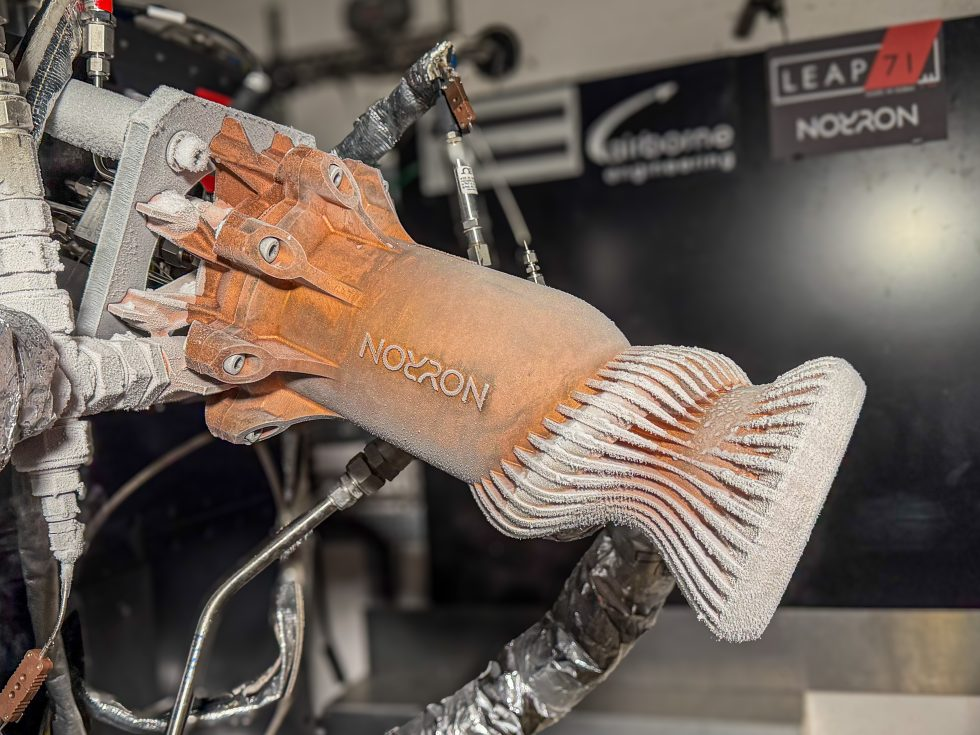
\includegraphics[height=\FigH, trim=120 0 40 0, clip]{images/leap71_engine.jpg}\\[-1pt]
		{\small (a)}
	\end{tabular}\hspace{2mm}%
	\begin{tabular}[b]{@{}c@{}}
		\resizebox{!}{\FigH}{\begin{tikzpicture}[font=\scriptsize\rmfamily, x=1cm, y=1cm,
				arr/.style={-{Stealth[length=1.5mm]}, line width=0.6pt}]
				% ---- cross-section A-A (top)
				\begin{scope}[shift={(0.45,2.75)}, scale=1.25]
					\fill[black!12] (0,0) rectangle (2.55,1.12);
					\foreach \x in {0.2,1.05,1.9} {
						\shade[top color=UPCAccent!35, bottom color=red!45] (\x,0.14) rectangle ++(0.45,0.84);
						\draw[black!60] (\x,0.14) rectangle ++(0.45,0.84);
						\draw[dashed, black!70] (\x,0.4) -- ++(0.45,0);
					}
					\foreach \x in {0.35,0.85,1.35,1.85,2.35} \draw[arr, red!70!black] (\x,-0.35) -- (\x,0.02);
					\node[red!70!black] at (1.27,-0.5) {$q_w$ (hot-gas side only)};
					\node[align=left, anchor=west] at (2.65,0.8) {liquid-like};
					\node[align=left, anchor=west] at (2.65,0.28) {gas-like};
					\draw[black!50] (2.35,0.75) -- (2.65,0.8); \draw[black!50] (2.35,0.25) -- (2.65,0.28);
					\node[anchor=south] at (1.27,1.12) {section A--A: cooling channels};
				\end{scope}
				% ---- thrust chamber and nozzle (upper half), wall with coolant passage
				\def\inner{(0,1.05) -- (1.4,1.05) .. controls (2.0,1.05) and (2.1,0.55) .. (2.5,0.55)
					.. controls (2.9,0.55) and (3.4,1.0) .. (4.3,1.45)}
				\def\outer{(0,1.40) -- (1.4,1.40) .. controls (2.0,1.40) and (2.1,0.90) .. (2.5,0.90)
					.. controls (2.9,0.90) and (3.4,1.35) .. (4.3,1.80)}
				\fill[orange!12] (0,0) -- \inner -- (4.3,0) -- cycle;
				\draw[line width=0.9pt, black!70] \inner;
				\draw[line width=0.9pt, black!70] \outer;
				\draw[black!40] (0,0) -- (4.3,0);
				\node[orange!70!black, align=center] at (0.85,0.55) {hot combustion\\ gas};
				\draw[arr, orange!80!black] (0.25,0.15) -- (1.45,0.15);
				\draw[arr, UPCAccent, line width=0.9pt] (4.15,1.62) .. controls (3.4,1.18) and (2.9,0.72) .. (2.5,0.72)
				.. controls (2.1,0.72) and (2.0,1.22) .. (1.4,1.22) -- (0.15,1.22);
				\node[UPCAccent, align=center, anchor=west] at (4.35,1.75) {coolant in\\ ($P>P_c$,\\ $T<T_{pb}$)};
				\node[UPCAccent, anchor=south] at (0.55,1.42) {to injector};
				\draw[arr, red!70!black] (2.5,0.15) -- (2.5,0.50);
				\node[red!70!black, align=center] at (2.5,-0.18) {throat: peak $q_w$};
				\draw[dashed, black!50] (1.8,1.6) -- (1.8,0.85) node[pos=0,above] {A};
		\end{tikzpicture}}\\[-1pt]
		{\small (b)}
	\end{tabular}\hspace{2mm}%
	\begin{tabular}[b]{@{}c@{}}
		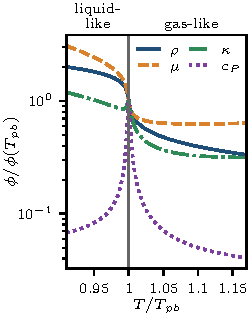
\includegraphics[height=\FigH]{images/co2_pseudoboiling_narrow.pdf}\\[-1pt]
		{\small (c)}
	\end{tabular}
	\caption{(a) Regeneratively cooled engine designed by LEAP~71; the frost on its surface is caused by the cryogenic propellant in the cooling passages (image:
		LEAP~71~\cite{LEAP71}). (b) Schematic of regenerative cooling at supercritical pressure through rectangular channels in the chamber wall; near the heated wall it crosses $T_{pb}$ and becomes gas-like, which can trigger heat-transfer deterioration~\cite{Pizzarelli2018,Nasuti2021,Urbano2013}. 
		(c) Thermophysical properties of CO$_2$ at 8~MPa across the pseudo-boiling temperature $T_{pb}=307.8$~K, normalized by their values at $T_{pb}$ (computed with CoolProp~\cite{CoolProp2014}).}
	\label{fig:regen}
\end{figure}


Despite substantial advances in understanding supercritical fluid flows, current knowledge remains largely confined to canonical configurations and restricted operating conditions \cite{Li2025}. High-fidelity simulations have revealed how strong thermophysical-property variations reshape turbulence and thermal transport \cite{Peeters2016,Guo2022}, yet their influence at higher Reynolds numbers, in complex geometries, and under nonuniform heating remains insufficiently understood. 
Square ducts, in particular, provide a canonical configuration for investigating how turbulence anisotropy and secondary motions interact with strong property variations (Figure~\ref{fig:duct}). 
These limitations are critical when predicting HTD, as it remains strongly dependent on operating conditions and flow configuration, with errors in the predicted peak wall temperature of up to 200~K near the critical pressure~\cite{Nasuti2021}. 
Likewise, pseudo-boiling can profoundly alter jet stability and development, yet its effects on entrainment and mixing remain poorly understood, limiting our ability to predict and optimize high-pressure injection and film cooling \cite{Lapenna2019,SharanBellan2021}.
Addressing these gaps is essential to exploiting supercritical-fluid properties while ensuring reliable thermal performance.

\begin{figure}[t]
\centering
\begin{tikzpicture}
  \node[anchor=north west, inner sep=0] (B) at (0,0)
    {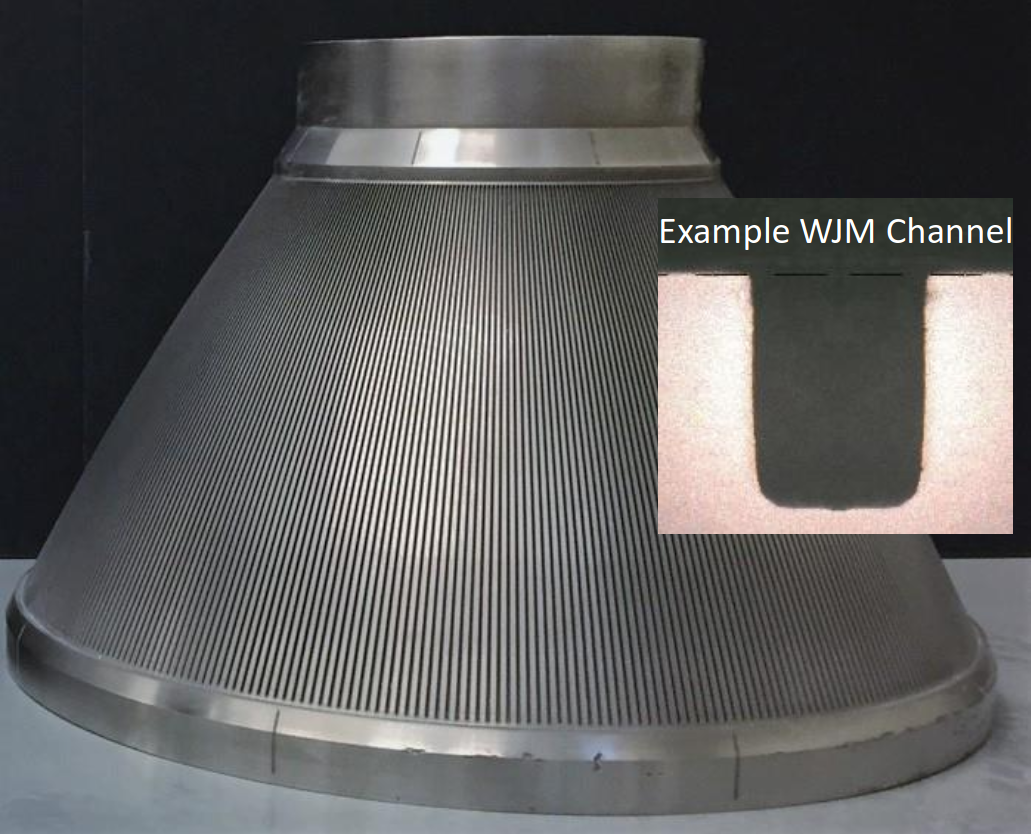
\includegraphics[height=6.3cm]{images/regen_NASA.png}};
  \node[anchor=north east, inner sep=0] (C) at (\textwidth,0)
    {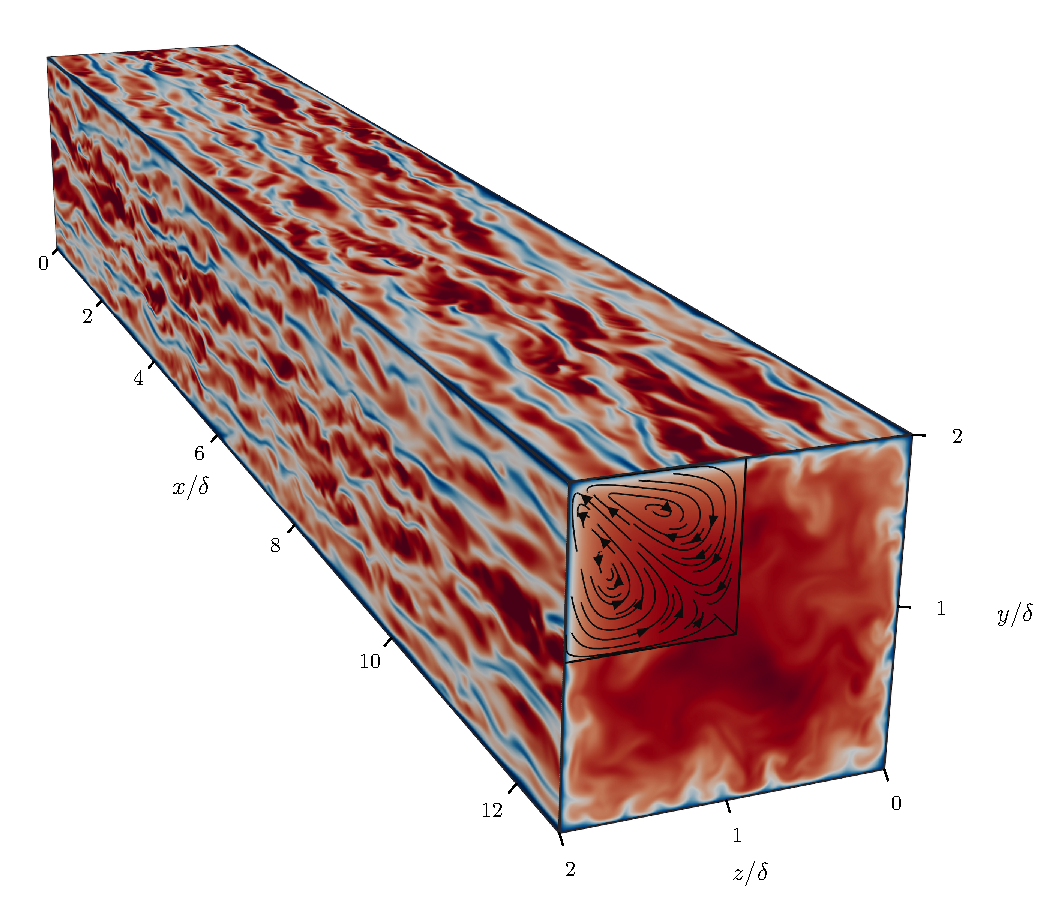
\includegraphics[height=6.3cm]{images/duct_L8.pdf}};
  \node[below=1pt of B] {\small (a)};
  \node[below=1pt of C] {\small (b)};
  \def\Bw{7.788cm}\def\Bh{6.3cm}\def\Cw{7.274cm}\def\Ch{6.3cm}
  \coordinate (I1) at ([xshift=0.639*\Bw, yshift=0.36*\Bh]B.south west);
  \coordinate (I2) at ([xshift=0.985*\Bw, yshift=0.745*\Bh]B.south west);
  \coordinate (K1) at ([xshift=0.515*\Cw, yshift=0.085*\Ch]C.south west);
  \coordinate (K2) at ([xshift=0.870*\Cw, yshift=0.515*\Ch]C.south west);
  \draw[red!80!black, line width=0.8pt] (I1) rectangle (I2);
  \draw[red!80!black, line width=0.8pt] (K1) rectangle (K2);
  \draw[red!80!black, densely dashed, line width=0.6pt] (I2) -- (K1 |- K2);
  \draw[red!80!black, densely dashed, line width=0.6pt] (I1 -| I2) -- (K1);
\end{tikzpicture}
\caption{(a) Coolant channels in a mid-scale Haynes~230 nozzle liner at NASA, with the cross-section of one channel (inset)~\cite{Gradl2019}. 
(b) DNS of turbulent square duct supercritical CO$_2$ flow in a square duct at 1.5 times the critical pressure, with walls hotter than $T_{pb}$ ($Re_b=12\,000$, $Re_\tau\approx300$, ongoing work). It shows instantaneous streamwise velocity on planes at $y^+\approx15$ from the walls and on the cross-section; the outlined quadrant shows the mean streamwise velocity and the streamlines of the secondary flow.}
\label{fig:duct}
\end{figure}


Beyond mean flow behavior, intermittent turbulent events can generate extreme wall-heat-flux fluctuations and localized thermal loads overlooked by conventional mean-based approaches.
Previous studies have characterized extreme wall events primarily in ideal-gas and constant-property turbulence \cite{Hack2021,Zhang2023}, but their underlying mechanisms and predictive precursors under supercritical conditions remain poorly understood.
In my preliminary investigations of turbulent CO$_2$ channel flow, I identified fluctuations exceeding ten times their root-mean-square value, associated with near-wall vortices transporting fluid of contrasting temperatures towards the wall (Figure~\ref{fig:extreme}a,b) [R3].
Drawing on these findings and my preliminary work at Stanford [R2, R3], information-theoretic causal analysis offers a promising approach to identifying the mechanisms and precursors of extreme events \cite{LozanoDuran2020,Massaro2023}.
Such advances could improve the prediction of critical operating conditions and the reliability of thermal systems.

\begin{figure}[t]
\centering
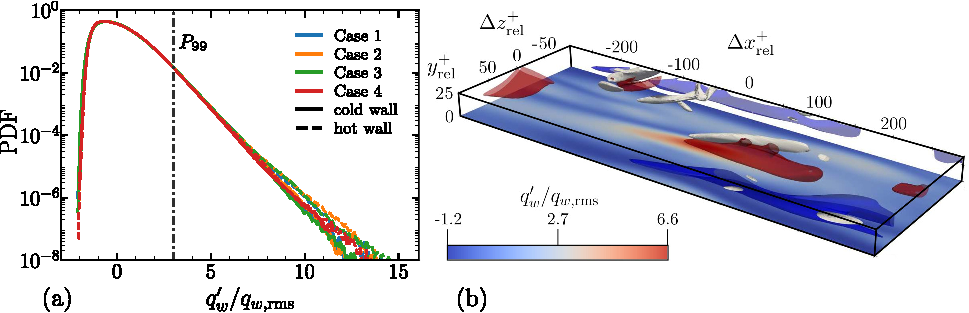
\includegraphics[width=\textwidth]{images/ctr_extreme_events.pdf}
\caption{Extreme wall-heat-flux events in supercritical CO$_2$ channel flow (three transcritical cases and a low-pressure reference) [R3]. (a) Probability density functions of the wall-heat-flux fluctuation normalized by its root-mean-square value, for all cases and both
walls. (b) Instantaneous extreme event at the cold wall of
case~1: wall heat flux (colormap), positive $Q$-criterion isosurfaces (white), and regions of hot (red) and cold (blue) fluid.}
\label{fig:extreme}
\end{figure}

Moreover, addressing these challenges requires increasingly sophisticated computational capabilities.
High-fidelity simulations must resolve strong property gradients, investigate increasingly demanding flow conditions, and capture sufficient statistics of rare events, imposing substantial computational costs.
These requirements motivate the continued development of efficient, scalable numerical methods capable of exploiting modern GPU-based supercomputing architectures.
Building on RHEA-X [J1], advances in real-fluid property evaluation, computational performance, and Lagrangian analysis will support these investigations.
By integrating fundamental flow physics, causal analysis of extreme events, and high-performance scientific computing, the proposed research program aims to advance the understanding and prediction of supercritical turbulent flows, ultimately contributing to more efficient and reliable energy and propulsion technologies.

\subsection{Research lines and objectives}\label{sec:lines}

The program is organized in three research lines, which follow closely the ones specified in the call(Figure~\ref{fig:lines}). 
This section highlights who my research background and experiences led to each line, its open problems, and the resulting objectives (O) and expected outcomes.

\begin{figure}[t]
\centering
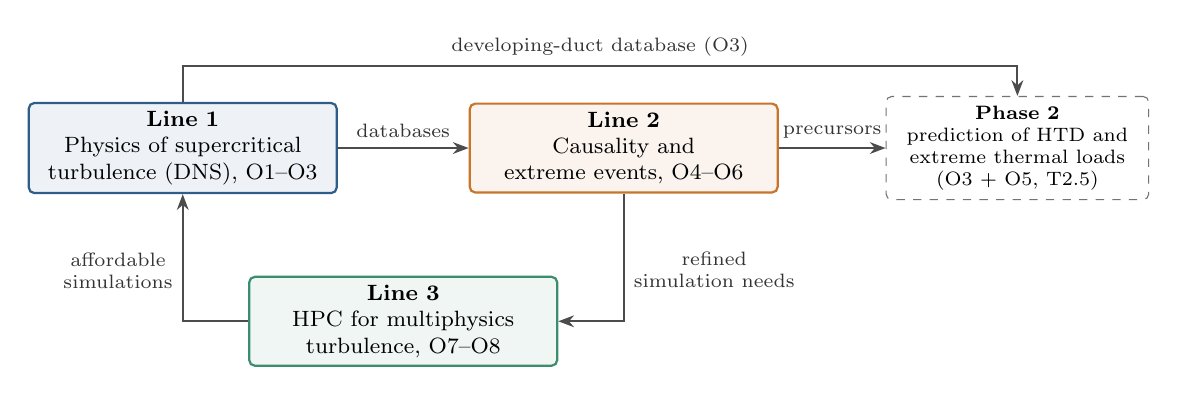
\begin{tikzpicture}[font=\footnotesize,
  box/.style={draw=#1, fill=#1!8, rounded corners=2pt, line width=0.8pt, align=center,
              text width=3.7cm, minimum height=1.05cm, inner sep=3pt},
  arr/.style={-{Stealth[length=2mm]}, line width=0.7pt, black!70},
  lab/.style={font=\scriptsize, align=center, black!80}]
  \definecolor{LA}{HTML}{2F5D8A}\definecolor{LB}{HTML}{C8742B}\definecolor{LC}{HTML}{3C8D6E}
  \node[box=LA] (L1) at (0,0) {\textbf{Line 1}\\ Physics of supercritical\\ turbulence (DNS), O1--O3};
  \node[box=LB] (L2) at (5.6,0) {\textbf{Line 2}\\ Causality and\\ extreme events, O4--O6};
  \node[box=LC] (L3) at (2.8,-2.2) {\textbf{Line 3}\\ HPC for multiphysics\\ turbulence, O7--O8};
  \node[draw=black!55, dashed, rounded corners=2pt, align=center, font=\scriptsize,
        text width=3.1cm, minimum height=1.05cm] (P) at (10.6,0)
        {\textbf{Phase 2}\\ prediction of HTD and\\ extreme thermal loads\\ (O3 + O5, T2.5)};
  \draw[arr] (L1) -- node[lab, above] {databases} (L2);
  \draw[arr] (L2) -- node[lab, above] {precursors} (P);
  \draw[arr] (L2.south) |- node[lab, pos=0.3, right] {refined\\ simulation needs} (L3.east);
  \draw[arr] (L3.west) -| node[lab, pos=0.7, left] {affordable\\ simulations} (L1.south);
  \draw[arr] (L1.north) |- ++(0,0.45) -| node[lab, pos=0.25, above] {developing-duct database (O3)} (P.north);
\end{tikzpicture}
\caption{Schematic of the scientific connection and dependencies between three research lines of this program.}
\label{fig:lines}
\end{figure}


%%%%%%%% CARLOS IS HERE %%%%%%%%%%%%%


\subsubsection{Line 1 -- Physics of supercritical turbulent flows}

My doctoral investigations demonstrated how pseudo-boiling can be exploited to enhance heat transfer and fundamentally modify turbulence in microconfined flows~\cite{Hurtan2025,Bernades2023,Bernades2025}.
In asymmetrically heated microducts, I showed that pseudo-boiling can trigger turbulence-like regimes under hydrodynamic conditions that remain laminar at low pressure, increasing the hot-wall Nusselt number by approximately $20\times$ with the same imposed temperature difference [J3, J4, J7].
In turbulent square ducts, I demonstrated that secondary-flow intensity can reach 4.6\,\% of the bulk velocity, approximately twice the upper bound reported for canonical ducts.
Moreover, changing the orientation of gravity altered secondary-flow intensity by more than 100\,\% and the hot- and cold-wall Nusselt numbers by up to 28\,\% and 63\,\%, respectively, despite variations below 10\,\% and 3\,\% in bulk and friction Reynolds numbers.
These findings revealed how buoyancy and pseudo-boiling interact to reorganize secondary motions and redistribute momentum, wall shear stress, and turbulent transport [J2, R1, C1].
During my research, I also revisited conventional DNS practices and established refined resolution and minimal-flow-unit guidelines for pseudo-boiling turbulence [J5, J6], demonstrating that grids reproducing first-order statistics within 2\,\% can nevertheless underestimate the intensity and wall proximity of the pseudo-boiling region, with substantial impact on turbulent intensities.
%Accurate characterization required finer near-wall resolution and wall-normal and cross-stream spacings below approximately 3.5 Kolmogorov and Batchelor scales [J5].
%I also reassessed the applicability of minimal flow-units, establishing their ability to reproduce near-wall turbulence while identifying limitations in capturing larger-scale motions [J6].

Informed by these contributions, this research line will pursue three complementary investigations, progressing from fundamental transport mechanisms to predictive correlations and the characterization of heat-transfer deterioration (HTD) in increasingly engineering-relevant configurations for space propulsion and thermodynamic cycle technologies:
\begin{enumerate}
	\item \textbf{Thermal transport mechanisms in asymmetrically heated ducts.}
	The first investigation will extend my previous analyses of asymmetrically heated channels and square ducts, where pseudo-boiling interacts with buoyancy and turbulence anisotropy.
	Although the organization of momentum transport and secondary motions has been characterized, the corresponding thermal mechanisms remain less thoroughly understood.
	Using existing DNS databases, I will investigate enthalpy and turbulent heat-flux budgets to quantify how buoyancy, secondary motions, and pseudo-boiling redistribute thermal energy and influence local heat transfer.
	In parallel, attention will be devoted to higher-order statistics and coherent turbulent structures associated with extreme wall-heat-flux events, especially at the heated wall.
	These analyses will establish a comprehensive physical interpretation of heat-transfer modulation and provide reference cases for the causal investigations developed in Line~2.
	
	\item \textbf{Generalized scaling laws and predictive correlations.}
	The second investigation, with simulations already underway (Figure~\ref{fig:duct}b), will examine high-pressure transcritical rectangular ducts with uniform perimeter heating, enabling systematic comparisons with canonical duct flows.
	By varying Reynolds number, thermophysical conditions, and aspect ratio, I will investigate the scaling of skin friction and Nusselt number, alongside momentum and thermal balances.
	Since existing correlations and variable-property transformations may lose accuracy under pseudo-boiling conditions \cite{Modesti2026,Li2025}, these simulations will support their critical assessment and the development of improved physics-based correlations and complementary data-driven models, an effort already initiated in collaboration with Prof.~Xiang Yang (Pennsylvania State University).
	The ambition is to establish broadly applicable predictive relationships that capture the combined influence of Reynolds number, turbulence anisotropy, buoyancy, and thermophysical conditions.
	
	\item \textbf{Heat-transfer deterioration in spatially developing flows.}
	The third investigation will extend the analysis towards spatially developing flows representative of supercritical cooling passages.
	Although previous studies have identified operating conditions associated with HTD, accurately predicting its onset remains challenging, and the underlying physical mechanisms continue to be debated \cite{Nasuti2021,Li2025}.
	Existing correlations can mispredict peak wall temperatures by up to 200~K near the critical pressure, illustrating the limitations of current predictive descriptions \cite{Nasuti2021}.
	I will perform DNS of spatially developing channels and square ducts heated from one side, progressively incorporating more representative heating conditions and cooling-passage geometries.
	These simulations will identify the mechanisms governing HTD onset, including the potentially synergistic influence of buoyancy, secondary motions, and the evolving thermal boundary layer.
	The resulting databases will also provide a demanding assessment of the predictive relationships developed in the second investigation, identifying their limitations and guiding their extension towards deteriorated heat-transfer conditions.
\end{enumerate}
Together, these investigations pursue three complementary scientific objectives:
\begin{itemize}
	\item[\textbf{O1.}] Identify and quantify how pseudo-boiling, buoyancy, and secondary motions govern turbulent heat transfer and extreme wall-heat-flux events in asymmetrically heated ducts relevant to regenerative cooling and energy-conversion systems.
	
	\item[\textbf{O2.}] Establish generalized scaling laws for skin friction and heat transfer in supercritical flows, identifying physically motivated dimensionless parameters that capture the combined effects of Reynolds number and pseudo-boiling to develop improved predictive correlations.
	
	\item[\textbf{O3.}] Elucidate the mechanisms governing HTD onset in spatially developing, asymmetrically heated ducts, quantifying the influence of secondary motions and cooling-passage geometry on thermal deterioration.
\end{itemize}
The program will deliver openly accessible, highly curated DNS databases spanning different heating conditions (both asymmetric and perimeter heating), Reynolds-number effects, and spatially developing flows exhibiting HTD, establishing reference benchmarks for the research community.
These will underpin generalized scaling laws and improved skin-friction and Nusselt-number correlations, including the identification of new dimensionless parameters to potentially capture the combined effects of Reynolds number, turbulence anisotropy in rectangular ducts, buoyancy, and supercritical thermodynamic conditions.
The research will also seek to establish a comprehensive physical understanding of HTD onset, identifying its governing mechanisms and developing predictive criteria for its occurrence.
Ultimately, these contributions will provide a high-fidelity foundation for validating and improving lower-fidelity computational fluid dynamics (CFD) approaches (RANS and LES) and extending predictive capabilities towards increasingly complex, engineering-relevant geometries and operating conditions.

Depending on funding availability, a complementary investigation of supercritical jets and mixing layers may also be pursued.
Previous investigations have shown that pseudo-boiling can substantially modify shear-layer instability and jet development \cite{Lapenna2019,SharanBellan2021}, yet its influence on turbulent interfaces and entrainment remains poorly characterized.
Building on the existing capabilities of RHEA-X [J1], I will investigate interactions between liquid-like and gas-like streams of the same fluid, isolating pseudo-boiling effects from the additional complexities of multicomponent mixing and advancing the understanding of turbulent entrainment relevant to high-pressure injection and film cooling.
In the longer term, this framework could be extended to multispecies mixing and transcritical atomization, addressing the coupled thermodynamic and interfacial phenomena encountered in high-pressure propulsion systems \cite{JofreUrzay2021}.

\subsubsection{Line 2 -- Causality and extreme events in multiphysics turbulence}

Extreme events in turbulent flows, from severe storms and floods to localized thermal loads in engineering systems, often have consequences far beyond those suggested by average conditions.
Rare fluctuations can dominate critical transport processes and impose loads that conventional mean and root-mean-square statistics fail to capture~\cite{Guerrero2020}.
Understanding the mechanisms preceding such events and whether they can be anticipated is therefore essential for improving prediction and reliability.
Conventional approaches, such as conditional averaging, characterize the turbulent structures around extreme events but do not establish their causal relationships \cite{Hack2021,Zhang2023}.
During the 2026 Stanford Center for Turbulence Research Summer Program, I initiated an alternative approach combining event-conditioned Eulerian statistics, Lagrangian tracking, and transfer entropy to investigate extreme wall-heat-flux events in supercritical CO$_2$ turbulence [R2, R3].
These investigations revealed a sequence of near-wall turbulent motions preceding extreme thermal events and identified candidate precursors carrying predictive information.
Building on these findings, this research line will develop through two complementary activities:
\begin{enumerate}
	\item \textbf{Causality and prediction of extreme events in supercritical turbulence.}
	Already under development, this investigation combines the formalization of a non-stationary, event-conditioned Lagrangian information-theoretic framework with its application to extreme wall-heat-flux events.
	Extending the preliminary transfer-entropy analyses [R2, R3], the primary approach to be tested will be the incorporation of multivariate decompositions of unique, redundant, and synergistic information contributions \cite{MartinezSanchez2024}.
	Its application to the Line~1 databases will establish how pseudo-boiling influences extreme thermal events and their precursors.
	By the start of the Lector appointment, this work should have reached a mature stage.
	
	\item \textbf{Generalization of the causal analysis approach to multiphysics turbulent systems.}
	The framework will be applied to physically distinct problems.
	The first application will address microplastic--biogenic particle collisions and aggregation in ocean turbulence, drawing on my summer 2027 research stay with Prof.~Mona Rahmani at the University of British Columbia.
	A subsequent research stay at the Universit\`a del Salento with Prof.~Mario Di Renzo and Prof.~Donatella Passiatore will support its extension to extreme thermal events in hypersonic boundary layers.
	A prospective third international stay at the California Institute of Technology, hosted by Prof.~Adrián Lozano-Durán, will provide additional opportunities to consolidate and validate the methodology across turbulent flow regimes (see Section~\ref{sec:mobility}).
\end{enumerate}
The natural follow-up scientific objectives are:
\begin{itemize}
	\item[\textbf{O4.}] Develop and validate a non-stationary Lagrangian information-theoretic framework for assessing causal relationships and identifying predictive precursors of rare turbulent events.
	\item[\textbf{O5.}] Identify the causal mechanisms and precursors of extreme events in supercritical turbulence and evaluate their predictive value across thermophysical and buoyancy regimes.
	\item[\textbf{O6.}] Demonstrate the framework's generality through applications to particle interactions in ocean turbulence and extreme thermal events in compressible and hypersonic flows.
\end{itemize}
The expected deliverables include an open-source, validated Lagrangian causality framework, benchmark cases for rare-event analysis, and physically interpretable predictive indicators of extreme wall-heat-flux events.
Its testing across different multiphysics turbulent flows will establish a high-impact transferable methodology for investigating and anticipating extreme events.

\subsubsection{Line 3 -- High-performance computing for high-fidelity simulation of complex turbulent flows}

RHEA-X [J1] is the computational code for the simulations in Line~1 and 2. 
Improving it is a natural next step as these investigations move towards larger and more complex simulations and research goals. 
Additionally, this line of work also serves a broader goal of establishing RHEA-X as a reference tool for high-fidelity CFD by improving its performance while maintaining reproducibility, and enabling researchers to add physical models and diagnostics through documented interfaces that reuse optimized GPU routines.
I co-developed RHEA-X, the successor to the open-source RHEA solver~\cite{RHEASoftware}, and led its port to distributed GPUs. 
The port retains a common C++ source for CPU and GPU (\href{https://www.openacc.org/}{OpenACC}) execution, keeps flow fields resident on the device, and uses GPU-aware MPI for halo exchanges. 
Benchmarks on different supercomputers (such as MareNostrum~5 at the \href{https://www.bsc.es/}{Barcelona Supercomputing Center (BSC)} and the Netherlands' national supercomputer \href{https://www.surf.nl/en/services/compute/snellius-the-national-supercomputer}{Snellius}) demonstrated speedups of up to $70\times$ over CPU execution and strong-scaling efficiencies of up to $97\,\%$ on as many as 64 GPUs [J1]. 
Building on this foundation, I plan on advancing the following topics:
\begin{enumerate}
	\item \textbf{Systematic kernel optimization across CPUs and GPUs.}
	I will benchmark different optimization strategies such as optimized data layout, cache reuse, kernel fusion and splitting, and asynchronous computation on representative DNS workloads. Comparisons across different architectures and paradigms (such as \href{https://www.khronos.org/sycl/}{SYCL}) will establish which optimizations transfer across architectures and which depend on the hardware or workload. 
	I will document their effects on runtime, memory use, scaling and agreement in flow statistics, with reproducible cases that other CFD developers can use to test the same choices.
	
	\item \textbf{Reliable substitution of costly physical models with surrogates.}
	I will establish a procedure for when a surrogate can replace a computationally demanding model. The first demonstration builds on [R4], where I am contributing to a surrogate model trained on CoolProp data~\cite{CoolProp2014} to replace selected property evaluations based on the Peng--Robinson equation of state~\cite{PengRobinson1976}. 
	For Line~1, I will quantify the gains in runtime and device memory alongside the errors in thermophysical properties and their gradients near pseudo-boiling, and assess how these errors affect wall heat flux and turbulent heat transport.
	
	\item \textbf{Guidelines for integrating new physical models and diagnostics.}
	I will develop documented C++ interfaces, implementation examples and verification cases that let contributors reuse the solver's accelerated capabilities. The guidelines will show how to implement a module, verify its results on CPUs and GPUs, and measure its cost in a full DNS. 
	For Line~2, I plan to demonstrate this approach with on-device Lagrangian tracking and in-situ event detection, testing how much trajectory output can be reduced while preserving the precursor statistics needed for extreme-event analysis.
\end{enumerate}
The aim of these contributions is to make it faster to add and test new physics in high-fidelity CFD. 
The optimization benchmarks will guide implementation choices, the surrogate procedure will establish when a cheaper model is accurate enough for the scientific question, and the integration guidelines will make both accessible to contributors. 
This foundation could also support longer-term investigations of high-speed supercritical flows, including shock interactions and multicomponent mixing, with reacting flows and finite-rate chemistry as subsequent extensions.
Therefore, two main objectives are established in this research line:
\begin{itemize}
	\item[\textbf{O7.}] Establish reproducible methods for optimizing DNS kernels across accelerated HPC architectures and for validating GPU-friendly surrogate replacements against the flow observables of interest.
	\item[\textbf{O8.}] Enable researchers to integrate and verify GPU-capable models and diagnostics through documented interfaces.
\end{itemize}

The deliverables will be versioned open-source releases of RHEA-X, reproducible benchmarks, and implementation guides with verified examples. 
These resources will support simulations in Lines~1 and~2, and the generation of documented datasets for physical analysis and data-driven modeling. 
The feasibility of this line also builds on six previous successful competitive supercomputing allocations (described in the HAP), two MareNostrum hackathons, ongoing collaboration with Xavier Álvarez-Farré (SURF), and technical exchanges with Lucas Gasparino (BSC) and Filippo Spiga (NVIDIA). 
The shared code and benchmarks will also support joint development and validation during the planned international research stays (Section~\ref{sec:mobility}).
Besides participating in further hackathons and continuing to apply for national allocations through the Spanish Supercomputing Network (RES), I plan to leverage this experience to apply for EuroHPC allocations, with the aim of scaling RHEA-X towards exascale performance.
Quantum computing also sparks my curiosity, and its feasibility for CFD, even as a partial offload, is a potential topic to explore in the long term~\cite{Bharadwaj2023}.

\Needspace{6\baselineskip}
\subsection{Work plan, timeline and risks}\label{sec:workplan}
The plan covers six years, from September 2027 to August 2033, with Year~1 corresponding to
the academic year 2027--28. The program develops gradually, from canonical configurations to
engineering-relevant conditions and from understanding to prediction: Line~1 moves from thermal
transport in asymmetrically heated ducts to scaling laws under perimeter heating and to HTD onset
in developing flows, with free shear flows depending on funding; Line~2 from a framework expected
to be mature at the start of the contract to its application to other multiphysics flows; and
Line~3 from kernel optimization and surrogates to documented interfaces and scaling towards
exascale. Scientifically, it is divided into two phases, consistent with the
intermediate evaluation of the contract: \textbf{Phase~1 (years 1--3), foundations}:
databases, validation and generalization of the causal framework, and optimized solver; and
\textbf{Phase~2 (years 4--6), prediction}: predictive criteria for HTD onset and extreme events,
engineering correlations and, if funding allows, free shear flows. In parallel, the Lector position
provides the framework to build an independent research program within GReCEF, in three
stages:
\begin{itemize}
  \item \textbf{Establishment (Y1--Y2, 2027--29):} integration into GReCEF, initial funding,
  continued publication as first author, first doctoral recruitment, the Salento stay and the first proposal as principal
  investigator.
  \item \textbf{Development (Y3--Y4, 2029--31):} execution of the first independent project,
  if funded; a small team of two doctoral students and master's students; the stay at
  Caltech.
  \item \textbf{Consolidation (Y5--Y6, 2031--33):} research leadership, the ERC Starting Grant
  proposal, follow-up funding, and research accreditation towards stabilization.
\end{itemize}
The work is organized in five work packages (WPs).

\paragraph{WP1 -- Supercritical turbulence databases (Line~1; O1--O3; Y1--Y6).} Carried out
mainly by doctoral student~1, under my supervision and co-supervision within GReCEF.
\emph{Tasks:} T1.1 thermal budgets, higher-order statistics and extreme events in the existing
asymmetrically heated databases (O1), and rectangular ducts with uniform perimeter heating at
varying Reynolds number, thermophysical conditions and aspect ratio (O2; Y1--Y3); T1.2 spatially
developing channels and square ducts heated from one side, with progressively more representative
heating conditions and geometries, to identify the mechanisms of HTD onset (O3; Y2--Y4); T1.3
scaling laws, correlations and complementary data-driven models, continuing the work initiated
with Penn State (O2; Y1--Y5); T1.4, depending on funding, single-fluid jets and mixing layers
across pseudo-boiling (tentatively Y5--Y6).
\emph{Outcomes:} open databases for asymmetric heating, perimeter heating and developing flows,
3--4 journal articles and doctoral thesis~1.

\paragraph{WP2 -- Causality and extreme events (Line~2; O4--O6; Y1--Y6).} Led by me.
\emph{Tasks:} T2.1 validation on benchmark cases and open-source release of the Lagrangian
framework, expected to be mature at the start of the contract (O4; Y1--Y2); T2.2 extreme
wall-heat-flux events in the existing and new WP1 databases and precursor-based prediction (O5;
Y1--Y4); T2.3 microplastic--biogenic particle aggregation in ocean turbulence, from the results
of the UBC stay, with ICM-CSIC (O6; Y1--Y3); T2.4 extreme thermal events in compressible and
hypersonic boundary layers, from the Salento stay, and validation across flow regimes during the
prospective Caltech stay (O6; Y1--Y3); T2.5 prediction of HTD onset combining the
framework with the WP1 developing-flow databases (O3, O5; Y4--Y6).
\emph{Outcomes:} 3--4 journal articles, an open-source causality code and joint articles with
the host groups.

\paragraph{WP3 -- Solver performance and extensibility (Line~3; O7, O8; Y1--Y6).}
\emph{Tasks:} T3.1 kernel optimization and reproducible benchmarks across CPUs, GPUs and
programming paradigms, prepared and tested in BSC hackathons (O7; Y1--Y3); T3.2 procedure to
replace costly models with surrogates, validated against flow observables [R4] (O7; Y1--Y3);
T3.3 documented interfaces and guidelines, demonstrated with on-device Lagrangian tracking and
in-situ event detection for WP2 (O8; Y2--Y4); T3.4 EuroHPC applications and scaling towards
exascale (O7; Y2--Y6). Bachelor's and master's theses at the EEBE contribute to T3.1--T3.3;
doctoral student~2 (Phase~2) can take T3.3--T3.4 or T2.5.
\emph{Outcomes:} versioned open-source releases, implementation guides with verified examples,
1--2 articles and the computing allocations required by WP1 and WP2.

\paragraph{WP4 -- Resources, group building and management (Y1--Y6).} Applications for
funding and computing time (Section~\ref{sec:resources}); recruitment of doctoral students
1 (Y2) and 2 (Y3--Y4); Year-3 self-assessment; research accreditation (Y5--Y6).

\paragraph{WP5 -- Mobility, collaborations and dissemination (Y1--Y6).} Stays and
collaborations (Section~\ref{sec:mobility}) and dissemination
(Section~\ref{sec:dissemination}).

\begin{center}\small
\begin{tabularx}{\textwidth}{@{}p{0.8cm}p{1.35cm}X@{}}
\toprule
\textbf{Mil.} & \textbf{Year} & \textbf{Milestone} \\
\midrule
M1 & Y1 & Causality framework validated on benchmark cases; publication of the square-duct and CTR work [R1, R3]; Salento stay; predoctoral applications for doctoral student~1. \\
M2 & Y2 & First proposal as principal investigator (\emph{Generaci\'on de Conocimiento}, Tipo~A) submitted; doctoral student~1 recruited; open-source causality code released; application for the Caltech stay. \\
M3 & Y3 & First open database (O2); optimized solver release; Caltech stay; start of the independent project, if funded; Year-3 self-assessment. \\
M4 & Y4 & Developing-flow HTD database (O3); doctoral student~2 recruited. \\
M5 & Y5 & First predictive criteria for HTD onset (O3, O5); ERC Starting Grant proposal in preparation; application for research accreditation. \\
M6 & Y6 & ERC Starting Grant proposal submitted; follow-up national proposal; defense of doctoral thesis~1. \\
M7 & Y6 & Exploratory free-shear results, if funded (T1.4); consolidated independent program on supercritical turbulence and extreme events. \\
\bottomrule
\end{tabularx}
\end{center}

\begin{figure}[H]
\centering
\definecolor{GLineA}{HTML}{2F5D8A}%
\definecolor{GLineB}{HTML}{C8742B}%
\definecolor{GLineC}{HTML}{3C8D6E}%
\definecolor{GCross}{HTML}{8C96A0}%
\definecolor{GFund}{HTML}{6B4C9A}%
\definecolor{GDec}{HTML}{C0392B}%
\begin{ganttchart}[
    hgrid={*1{black!10}},
    vgrid={*3{black!10, dashed}, *1{black!35}},
    x unit=0.48cm, y unit title=0.5cm, y unit chart=0.47cm,
    time slot format=simple,
    canvas/.append style={draw=black!35, line width=0.4pt},
    title/.append style={draw=black!35, fill=MSBlue!12},
    title label font=\scriptsize\bfseries\color{MSBlue},
    title height=1,
    bar height=0.5, bar top shift=0.25,
    bar/.append style={draw=none, rounded corners=1.5pt},
    bar label font=\scriptsize,
    bar label node/.append style={align=right},
    milestone/.append style={fill=GFund, draw=none},
    milestone label font=\scriptsize,
    milestone height=0.5, milestone top shift=0.25
  ]{1}{24}
  \gantttitle{Establishment}{8}\gantttitle{Development}{8}\gantttitle{Consolidation}{8}\\
  \gantttitle{Y1 27--28}{4}\gantttitle{Y2 28--29}{4}\gantttitle{Y3 29--30}{4}\gantttitle{Y4 30--31}{4}\gantttitle{Y5 31--32}{4}\gantttitle{Y6 32--33}{4}\\
  \ganttbar[bar/.append style={fill=GLineA}]{T1.1 Thermal budgets, scaling}{1}{12}\\
  \ganttbar[bar/.append style={fill=GLineA}]{T1.2 Developing flows (HTD)}{5}{16}\\
  \ganttbar[bar/.append style={fill=GLineA!60}]{T1.3 Correlations, models}{1}{20}\\
  \ganttbar[bar/.append style={fill=GLineA!25, draw=GLineA, dashed}]{T1.4 Free shear (if funded)}{17}{24}\\
  \ganttbar[bar/.append style={fill=GLineB}]{T2.1 Validation, release}{1}{8}\\
  \ganttbar[bar/.append style={fill=GLineB}]{T2.2 Extreme heat flux}{1}{16}\\
  \ganttbar[bar/.append style={fill=GLineB!60}]{T2.3 Ocean (UBC, ICM)}{1}{12}\\
  \ganttbar[bar/.append style={fill=GLineB!60}]{T2.4 Hypersonic BL, validation}{2}{12}\\
  \ganttbar[bar/.append style={fill=GLineB!40}]{T2.5 HTD prediction}{13}{24}\\
  \ganttbar[bar/.append style={fill=GLineC}]{T3.1--T3.2 Kernels, surrogates}{1}{12}\\
  \ganttbar[bar/.append style={fill=GLineC!60}]{T3.3--T3.4 Interfaces, EuroHPC}{5}{24}\ganttnewline[black!60]
  \ganttbar[bar/.append style={fill=GFund!35}]{ALECTORS, GReCEF projects}{1}{6}\\
  \ganttbar[bar/.append style={fill=GFund!35}]{PID Tipo A: prep., subm., decision}{2}{4}%
  \ganttmilestone[inline]{}{6}%
  \ganttmilestone[inline, milestone/.append style={fill=GDec}]{}{9}\\
  \ganttbar[bar/.append style={fill=GFund}]{PID project (if funded)}{10}{21}%
  \ganttbar[inline, bar/.append style={fill=GFund!25, draw=GFund, dashed}]{}{22}{24}\\
  \ganttbar[bar/.append style={fill=GFund!35}]{ERC StG: prep., submission}{17}{20}%
  \ganttmilestone[inline]{}{21}\\
  \ganttmilestone{Follow-up national proposal}{22}\\
  \ganttbar[bar/.append style={fill=GCross}]{Stays (Salento, Caltech)}{3}{3}%
  \ganttbar[inline, bar/.append style={fill=GCross!40, draw=GCross, dashed}]{}{10}{11}\\
  \ganttbar[bar/.append style={fill=GFund!35}]{PhD 1: funding, thesis, defense}{1}{4}%
  \ganttbar[inline, bar/.append style={fill=GLineA!70}]{}{6}{22}%
  \ganttmilestone[inline, milestone/.append style={fill=MSBlue}]{}{23}\\
  \ganttbar[bar/.append style={fill=GFund!35}]{PhD 2 (FPI, if funded)}{10}{12}%
  \ganttbar[inline, bar/.append style={fill=GLineA!70}]{}{13}{24}\\
  \ganttmilestone[milestone/.append style={fill=GDec}]{Year-3 self-assessment}{12}\\
  \ganttbar[bar/.append style={fill=GFund!35}]{Research accreditation (AQU)}{17}{20}%
  \ganttmilestone[inline]{}{21}
\end{ganttchart}
\caption{Timeline by quarters (Y1 = 2027--28). Upper block: scientific tasks
(\textcolor{GLineA}{$\blacksquare$}~Line~1, \textcolor{GLineB}{$\blacksquare$}~Line~2,
\textcolor{GLineC}{$\blacksquare$}~Line~3). Lower block: light purple bars, proposal preparation
or applications; purple diamonds, submissions; red diamonds, expected funding decision and
evaluation; solid bars, execution and doctoral theses. In both blocks, dashed bars indicate
conditional or optional periods. The UBC stay (summer 2027) precedes Y1. All dates after Y1 are indicative and depend
on future calls and on successful evaluation.}
\end{figure}

\paragraph{Risk management.}
\begin{center}\small
\begin{tabularx}{\textwidth}{@{}>{\raggedright\arraybackslash}p{4.4cm}X@{}}
\toprule
\textbf{Risk} & \textbf{Mitigation} \\
\midrule
Not eligible for Tipo~A in 2028 & Participation in a GReCEF proposal as co-principal investigator or team member; independent proposal in the next suitable call. \\
Tipo~A proposal not funded (2029) & WP1 continues with initial funding, existing databases and computing allocations; resubmission with Phase~1 results; doctoral students funded through FI, FPU or UPC grants, independent of the project. \\
Doctoral student~1 not recruited in Y2 & T1.1 started by me and by master's theses; recruitment moved to the next call; T1.4 postponed. \\
Insufficient computing allocation & Simulation campaigns prioritized by objective (O1--O2 before O3); reduced domains justified by the minimal-flow-unit criteria [J6]; national and UPC resources for smaller cases. \\
Estimators unreliable for rare events (O4) & Larger event ensembles from longer DNS; fall-back to conditional statistics and conditional POD~\cite{Martin2025}, which still identify precursors and test their predictive value, although not their causality (O5 in part). \\
Caltech stay not funded & Self-funded further stays at UBC and Salento (T2.3, T2.4), of at least three months in total to reach the nine required for accreditation, scheduled in agreement with the Department to concentrate my teaching in one of the semesters; the collaborations with Caltech and Stanford continue remotely. \\
ERC Starting Grant not funded & Resubmission at the next eligible call; the follow-up national proposal ensures continuity. \\
\bottomrule
\end{tabularx}
\end{center}

\subsection{Funding, resources and career development}\label{sec:resources}
\paragraph{Starting point.} The ERC Starting Grant SCRAMBLE, which currently funds my
postdoctoral position, and the infrastructure of GReCEF cover the first months of WP1--WP3.

\paragraph{Independent output before the first project.} Until a project as principal
investigator starts (2029 at the earliest), the research does not depend on new funding: it
builds on the existing databases, the RHEA-X solver and yearly competitive computing
allocations. During Y1--Y2 I will keep publishing as first and corresponding author in the
lines I lead: the square-duct and causality manuscripts [R1--R3], the causal framework
(T2.1) and the joint work of the UBC and Salento stays, with a target of at least two journal
articles per year. This record of independent output is the basis of the first proposal as
principal investigator and, later, of the ERC Starting Grant proposal.

\paragraph{Funding strategy.} The Lector position provides the institutional framework to
apply for competitive funding as principal investigator. No funding has yet been awarded for
this plan; the applications below are planned, subject to eligibility and successful
evaluation, and each one supports specific objectives of Section~\ref{sec:research}.
\begin{itemize}
  \item \textbf{Initial funding (2027--28).} The UPC ALECTORS program for newly appointed
  Lector staff, subject to the call conditions, to start WP1--WP3; contribution to the
  ongoing projects of GReCEF, in a role that keeps me eligible to submit an independent
  proposal in 2028; and competitive predoctoral applications for doctoral student~1 (AGAUR
  FI Joan Or\'o, FPU of the Ministry and UPC predoctoral grants).
  \item \textbf{Independent national funding (2028--29).} An AEI \emph{Proyecto de
  Generaci\'on de Conocimiento}, Tipo~A, prepared in the first half of 2028 and submitted in
  late 2028, subject to the eligibility rules of that call. The objective is to secure a three-
  or four-year project, with execution in 2029--2032/33, on supercritical duct turbulence and
  the causal prediction of extreme heat-transfer events (O1--O3, O5): computing campaigns,
  doctoral research, collaborations and dissemination. An associated predoctoral contract
  (FPI) for doctoral student~2 will be requested where the call allows it. AGAUR
  \emph{Doctorats Industrials} with companies in the energy and space sectors will also be
  considered.
  \item \textbf{Research development (2029--31).} Execution of the first independent project,
  if funded, and complementary collaborative funding where compatible with it: Horizon
  Europe Cluster~5 (Climate, Energy and Mobility) consortia, \emph{Redes de Investigaci\'on}
  with Spanish groups on supercritical and compressible flows, and Marie
  Sk\l{}odowska-Curie Postdoctoral Fellowships and Doctoral Networks hosted at the UPC.
  \item \textbf{Major international funding (2031--33).} An ERC Starting Grant proposal,
  prepared in 2031--32 and submitted in 2032 (2033 as an alternative), subject to the
  eligibility of the corresponding call; and a follow-up national proposal to ensure the
  continuity of the doctoral projects.
\end{itemize}
\paragraph{Long-term direction.} By the end of the contract, the program aims to predict the
consequences of strong property variations in engineering flows: both the transport
enhancement that the applications seek and the HTD and extreme thermal loads that limit them, in
regenerative cooling channels and sCO$_2$ heat exchangers~\cite{Pizzarelli2018,Ahn2015}. The
same capabilities lead naturally to high-speed aerothermodynamics, where extreme wall heat
fluxes, large property variations and thermochemical effects
coexist~\cite{Urzay2018,DiRenzoUrzay2021,Passiatore2022}. This extension continues my work on
variable-property turbulence, extreme thermal events and GPU-accelerated high-fidelity CFD. It
starts with T2.4 at the Universit\`a del Salento, whose hosts have studied hypersonic
boundary layers~\cite{DiRenzoUrzay2021,Passiatore2022}, is consolidated during the Caltech stay, and
is in line with the department's priority on compressible flows. Extending RHEA-X to high-speed
supercritical flows, with shock interactions and multicomponent mixing, is a longer-term development
(Line~3).

\paragraph{Engineering transfer.} From Phase~2 and beyond the contract, the program will carry its
results to engineering design in three steps. First, the DNS databases calibrate and validate the
models that engineering tools need: correlations and transformations (O2), turbulent Prandtl number
and wall models for RANS and LES, and data-driven models of velocity and temperature profiles.
Classical correlations lose accuracy near pseudo-boiling: they can mispredict the peak wall
temperature by up to 200~K near the critical pressure~\cite{Nasuti2021}, and those for
supercritical CO$_2$ cooling depend strongly on geometry and operating
conditions~\cite{Pitla1998}. Second, the real-fluid property surrogates of Line~3 [R4] will be
coupled to OpenFOAM, so that RANS and LES of real cooling passages and heat exchangers use the
thermophysics validated by DNS. Third, these tools will be applied to regeneratively cooled channels
produced by additive manufacturing, including wall roughness and conjugate heat transfer
(Figures~\ref{fig:regen}a and~\ref{fig:duct}a); to sCO$_2$ Brayton cycles, whose precoolers,
recuperators and compressor inlet operate near the pseudo-critical point~\cite{Ahn2015}; to
transcritical CO$_2$ heat pumps, whose gas coolers operate across pseudo-boiling; and to
supercritical organic Rankine cycles for waste-heat recovery. Waste heat accounts for more than half
of the global primary energy~\cite{Markides2025}, and the working fluids of these cycles are changing:
the EU F-gas Regulation phases out HFCs by 2050~\cite{FGas2024}, and the proposed EU restriction of
PFAS also covers most HFO working fluids~\cite{ECHA2025}. Line~2 adds design margins that account for
extreme events, through probabilistic limits on the wall temperature and precursor-based monitoring.
These activities will be carried out through industrial doctorates and contracts with companies in
the energy and space sectors (Section~\ref{sec:dissemination}).

The ERC Starting Grant is placed deliberately at the end of the contract. By then, the
proposal can build on the results of the first independent project, experience managing
competitive funding, doctoral supervision, an independent publication record, and the
collaborations established at UBC, Salento and Caltech. Its scientific question
will go substantially beyond the national project: from understanding supercritical turbulence
and extreme events to their causal prediction and control in real-fluid and high-speed flows
(see the long-term direction above).

\paragraph{Accreditation and stabilization.} Progression to a permanent Professor Agregat
position at the end of the six-year contract requires the research accreditation of AQU
Catalunya (\emph{acreditaci\'o de recerca}). The outputs, funding and supervision planned
above are aligned with its criteria; I will apply in Y5 and aim to obtain it before the end
of the contract. Since 2025, this accreditation also requires at least nine months of
accumulated research or teaching activity at universities or research centers other than the
one where the doctoral thesis was presented, counting only the postdoctoral
period~\cite{AQU2025}. As my thesis was presented at the UPC, the stays of
Section~\ref{sec:mobility} (UBC, 3 months; Salento, 3 months; Caltech, 6 months;
12 months in total, which leaves a margin over the minimum) are a necessary part of the plan, not an option. If the Caltech stay is not funded, self-funded further
stays at UBC and Salento will cover the months needed to reach the minimum (Section~\ref{sec:workplan}). The R3 certification will be considered as a complementary objective, subject
to its requirements; it is not a prerequisite for the plan.

\paragraph{Computing resources.} The DNS of WP1 require several million GPU hours per year. I will apply every year to the RES calls (MareNostrum~5, BSC) and, from year~2, to
the EuroHPC JU \emph{Regular} and \emph{Extreme Scale} calls, which give access to
pre-exascale and exascale systems. The collaboration with UBC provides access to Canadian
national systems through the Digital Research Alliance of Canada, as in the RAC-2026
allocation. This builds on six competitive allocations in 2023--2026, totaling more than 10
million core and GPU hours.

\paragraph{Software and data.} RHEA-X [J1] (open source, MPI + OpenACC) is the core solver of
WP1--WP3. Analysis uses Python and Julia, the thermophysical surrogate software [R4] and
CoolProp~\cite{CoolProp2014}. Databases are stored on the long-term storage of the HPC centers
and published in open repositories (Zenodo, Figshare+, BLASTNet [D1]).


\Needspace{6\baselineskip}
\subsection{Team, collaborations and dissemination}\label{sec:mobility}\label{sec:dissemination}
\subsubsection*{Doctoral supervision and team}
Teaching at the EEBE allows identifying motivated students early, and bachelor's and
master's theses will be the entry point to the research lines. I currently tutor a
curricular internship on extreme events in turbulent flows and co-supervised a bachelor's
thesis on supercritical duct flow. I aim to supervise two doctoral theses during the
contract, as director, with co-supervision within GReCEF or with international partners where
it adds expertise. Both will be financed through competitive predoctoral grants, and their
topics contribute directly to the objectives of Section~\ref{sec:research}:
\begin{enumerate}
  \item \textbf{Doctoral thesis 1 (Y2--Y6): high-fidelity databases of supercritical duct
  turbulence and heat-transfer deterioration} (WP1). Applications to AGAUR FI Joan Or\'o, FPU
  and UPC predoctoral grants in Y1, with recruitment in 2028--29, subject to funding and the
  requirements of the doctoral program.
  \item \textbf{Doctoral thesis 2 (Y3/Y4--): prediction of extreme heat-transfer events, or
  extensible GPU solvers with in-situ Lagrangian analysis, scaled towards exascale} (WP2 or WP3). Funding: FPI
  contract associated with the national project, if funded, or the next FI and FPU calls.
\end{enumerate}
Together with master's students and, where funding allows, a postdoctoral fellow (MSCA), they
form the small team that executes the independent project.
Master's theses (TFM) will address one task each, for instance benchmark cases for causal
analysis (T2.1), kernel optimization (T3.1) or surrogate integration (T3.2); bachelor's
theses (TFG) will address GPU acceleration of simple solvers and the thermodynamic analysis of
sCO$_2$ cycles (Section~\ref{sec:theses}).

\subsubsection*{Ongoing collaborations}
The following collaborations are already active, unless marked as prospective, and will continue mainly remotely, through shared
data and codes, regular meetings, co-supervision of students and joint publications; some of them
are reinforced by the stays described below.
\begin{itemize}
  \item \textbf{The Pennsylvania State University (USA)}, Prof.\ X.\ Yang: compact neural networks
  for wall-normal profiles, trained on our supercritical-flow databases (Line~1, O2; remote).
  \item \textbf{Center for Turbulence Research, Stanford University (USA)},
  \href{https://me.stanford.edu/people/sanjiva-lele}{Prof.\ S.\ Lele} and his research team, including
  A.\ Chandra: a strong international collaboration that will keep the program connected to research
  on supercritical fluids. It builds on the joint work with A.\ Chandra in the 2026 Summer Program,
  selected through a competitive call, on non-stationary transfer entropy for extreme wall-heat-flux
  events (Lines~1 and~2; remote).
  \item \textbf{Caltech and MIT (USA)}, Prof.\ A.\ Lozano-Dur\'an and \'A.\ Mart\'inez-S\'anchez:
  causality and Lagrangian information-theoretic frameworks for turbulence (Line~2, O4--O5; remote; stay at Caltech in 2029--30).
  \item \textbf{Stanford University (USA)}, group of Prof.\ M.\ Ihme: contribution of our databases
  to the BLASTNet machine-learning dataset [D1] (Line~1; remote).
  \item \textbf{University of British Columbia (Canada)}, Prof.\ M.\ Rahmani: causality in ocean
  turbulence and aggregation of microplastics, already active through the RAC-2026 GPU allocation
  (Line~2, O6; stay in 2027).
  \item \textbf{Universit\`a del Salento (Italy)}, Prof.\ M.\ Di Renzo and Prof.\ D.\ Passiatore:
  extreme wall-heat-flux events in hypersonic flows, started at the 2026 CTR Summer Program
  (Line~2, O6; stay in 2028).
  \item \textbf{Instituto Superior T\'ecnico, Lisbon (Portugal)}, Prof.\ C.\ B.\ da Silva
  (prospective; remote): turbulent/non-turbulent and turbulent/turbulent interfaces in flows with
  variable properties (Line~1, T1.4, depending on funding). His group has characterized these interfaces in jets and
  shear-free flows at high Reynolds numbers~\cite{Silva2018,Alves2025}; single-fluid transcritical
  jets have been simulated~\cite{Lapenna2019,Ream2025}, but their interfaces have not been analyzed,
  although pseudo-boiling changes density, viscosity and diffusivity precisely across them.
  \item \textbf{SURF (the Netherlands)}, X.\ \'Alvarez-Farr\'e: ongoing collaboration on RHEA-X,
  complemented by technical exchanges with F.\ Spiga (NVIDIA) (Line~3, O7--O8; remote).
  \item \textbf{Local partners:} the Institut de Ci\`encies del Mar (ICM-CSIC), on microplastics and
  biofilms (O6), and the Barcelona Supercomputing Center, through the GPU hackathons and technical exchanges with L.\ Gasparino (O7).
  %\item \textbf{Prospective collaborations.} \MAYBE{Smart Ocean Peniche (Portugal): R\&D projects in ocean engineering.}
\end{itemize}

\paragraph{Collaborations within the UPC.} I also aim to build collaborations within the UPC that
complement the numerical program: with J.\ Calafell (Department of Fluid Mechanics), who develops
data-driven wall models with graph neural networks, on machine-learning models trained on the DNS
databases (O2) and on wall-modeled LES for the engineering transfer; and with J.\ Casals-Terr\'e
(Department of Mechanical Engineering) and M.\ Jofre (Department of Network Engineering), co-authors
of the data-informed analysis of experiments on microconfined transcritical turbulence [J7], on
experiments that validate the simulations.

\subsubsection*{Planned mobility}
Three postdoctoral stays develop the research lines with these groups and, together, provide the
nine months of mobility required for the research accreditation (Section~\ref{sec:resources}).
\begin{itemize}
  \item \textbf{University of British Columbia (Canada), summer 2027, 3 months, before the
  contract.} Host: \href{https://chbe.ubc.ca/mona-rahmani/}{Prof.\ Mona Rahmani}. Lagrangian
  causality applied to the aggregation of microplastics in ocean turbulence (Mitacs Globalink
  Research Award; T2.3).
  
  \item \textbf{Universit\`a del Salento (Italy), first half of 2028 (Y1), 3 months.} Hosts:
  \href{https://www.unisalento.it/scheda-utente/-/people/mario.direnzo}{Prof.\ Mario Di Renzo}
  and \href{https://www.unisalento.it/scheda-utente/-/people/donatella.passiatore}{Prof.\
  Donatella Passiatore}. Extreme wall heat flux in compressible and hypersonic boundary layers (T2.4), with
  joint articles and preliminary results for the national proposal. The Department of Fluid
  Mechanics has agreed to concentrate my teaching in one semester. The stay is limited to
  three months so that, together with the UBC stay, it keeps me eligible for the José
  Castillejo program for the Caltech stay.
  
  \item \textbf{Caltech (USA), 2029--30 (Y3), 6 months,
  prospective.} Hosted by Prof.\ A.\ Lozano-Dur\'an, whose expertise in causality is central to Line~2. The stay extends T2.4 and the causal framework of WP2, and prepares the collaborations of the ERC proposal. Two funding routes are planned,
  with applications in Y2 and subject to the host's agreement and compatibility with
  teaching: the Fulbright Portugal research grant (\emph{Bolsa Fulbright para
  Investiga\c{c}\~ao}, 4--6 months, open to all areas), and the José Castillejo program of the
  Spanish Ministry, either in its general track or in its Fulbright track, which adds a minimum
  score in the scientific evaluation and a limited number of grants.
\end{itemize}

\subsubsection*{Open science, transfer and dissemination}
\begin{itemize}
  \item \textbf{Databases and code:} the WP1 databases (Zenodo, Figshare+, BLASTNet), the
  causality code (WP2) and versioned releases of RHEA-X (WP3), following the FAIR principles.
  \item \textbf{Journals:} \emph{J.\ Fluid Mech.}, \emph{Phys.\ Rev.\ Fluids}, \emph{Int.\ J.\
  Heat Mass Transfer}, \emph{Phys.\ Fluids}, \emph{Comput.\ Phys.\ Commun.}
  \item \textbf{Conferences and programs:} THMT-27 and EFDC3 (2027, scheduled); the CTR Summer
  Program (biennial, next edition in 2028); the Madrid Summer School on Turbulence (2029,
  tentative); APS-DFD, ETMM, TSFP and the European Turbulence Conference.
  \item \textbf{Transfer:} reference data and predictive tools for the design of cooling
  channels and sCO$_2$ heat exchangers; industrial doctorates and contracts through the UPC
  transfer services. Spain invests directly in space transportation, with \texteuro{}40.5
  million for the development of the first Spanish small-satellite launcher~\cite{CDTI2024},
  and ESA's FLPP pursues high-thrust liquid propulsion~\cite{ESA2026}; Spanish companies
  developing liquid-rocket engines, such as PLD Space and the Barcelona-based Pangea Aerospace,
  which designs regeneratively cooled engines with real-fluid models~\cite{Esnault2021}, are
  prospective partners.
  \item \textbf{Outreach:} UPC open days, the \emph{Setmana de la Ci\`encia}, and initiatives
  that encourage girls to pursue engineering studies.
\end{itemize}

% =====================================================================
\section{Teaching plan}\label{sec:teaching}

\subsection{Teaching background}
Since 2024--25 I have taught 180 class hours at the UPC, and in 2026--27 I teach the full
load of my contract (242 hours). At the EEBE, I have taught the laboratory of \emph{Fluid
Mechanics} (820013) every year since 2024--25 (eight groups, 120 hours), and in autumn
2026 I teach the full course of group M1 of \emph{Thermodynamics and Heat Transfer}
(820020), supporting the coordination of the subject in exam preparation, marking and
review. At the EPSEVG, I teach the laboratory of \emph{Fundamentals of Thermal
Engineering} (340038), and in spring 2027 I will coordinate \emph{Fluid Engineering}
(340058) and teach its two theory groups. Student surveys rated my Fluid Mechanics
laboratory groups at 4.6--4.8 out of 5 in 2025--26 S2, above the department, school and
university averages.

\subsection{Personal vision of teaching}
I see engineering teaching as training students to model a real system: to decide what
matters, write the balance that governs it, estimate the answer before computing it, and
check that the result makes physical sense. Thermodynamics, heat transfer and fluid
mechanics are well suited to this, because every concept can be tied to a device the
students know: a heat pump, a pumping installation, a car, a power cycle.

Three principles guide my teaching:
\begin{itemize}
  \item \textbf{Clarity and closeness.} I explain each session step by step and make sure
  the group has understood before moving on.
  \item \textbf{Feedback to learn, not only to grade.} I return individual comments on
  every laboratory report so that students improve progressively, which they highlight in
  the surveys. The same idea guides the exam reviews in Thermodynamics and Heat Transfer.
  \item \textbf{Current engineering in the classroom.} My industrial experience (thermal
  simulation at Continental, Formula Student aerodynamics) and my research on supercritical
  fluids and high-performance computing provide examples and computational tools that make
  the classical content relevant. For instance, an inverter-cooling case shows how
  conduction through solid components and convection at cooling surfaces together
  determine component temperatures.
\end{itemize}

Following a common classification of engineering studies, the subjects of the call play
different roles: \emph{core subjects} such as Fluid Mechanics and Thermodynamics and Heat
Transfer set the basis that later subjects assume, while \emph{specialized subjects} such
as Fluid Engineering, Thermal Engineering and Computational Fluid Mechanics extend this
basis to engineering applications. Core subjects should prioritize solid fundamentals and
working habits; specialized subjects should connect them to design decisions and to the
tools used in industry and research. Active learning, which has been shown to improve
student performance in science and engineering~\cite{Freeman2014}, will be introduced
progressively and coordinated with the other lecturers of each subject.

\subsection{Institutional context}\label{sec:context}
\paragraph{The EHEA framework.} Teaching at the UPC follows the European Higher Education
Area (EHEA), initiated with the Bologna Declaration in 1999 and implemented in Spain
through Royal Decree 1393/2007. Its central elements are the two-cycle structure
(bachelor's and master's degrees, followed by the doctorate), the European Credit Transfer
System (ECTS), in which one credit corresponds to 25--30 hours of student work, including
autonomous study, and competence-based learning. Bachelor's degrees in Spain have 240
ECTS. At the UPC, study plans are defined in terms of specific and generic competences
that must be assessed, with particular attention to autonomous learning, teamwork,
sustainability and foreign languages.

\paragraph{The EEBE.} The Barcelona East School of Engineering (EEBE) started in 2016--17
as the core of the Diagonal-Bes\`os Campus, with about 3,500 students and 400 teaching and
research staff at its opening. Its aim is to be a high-quality engineering hub for the
industry of the 21st century, combining teaching with research, innovation and knowledge
transfer. The EEBE offers seven bachelor's degrees (Biomedical, Energy, Materials,
Electrical, Industrial Electronics and Automatic Control, Mechanical, and Chemical
Engineering), several master's degrees, including the Master's Degree in Mechanical
Technologies, and doctoral programs. The bachelor's degrees share a common first block in
which \emph{Fluid Mechanics} (semester 3) and \emph{Thermodynamics and Heat Transfer}
(semester 4) are compulsory, so these subjects reach a large number of students from
different degrees. Each degree then builds on this block with its own specialized
subjects.

\paragraph{The EPSEVG.} The Vilanova i la Geltr\'u School of Engineering (EPSEVG) offers
bachelor's degrees in the industrial field. \emph{Fluid Engineering} is compulsory in the
Bachelor's Degree in Mechanical Engineering and optional in the degrees in Electrical
Engineering and in Industrial Electronics and Automatic Control Engineering.

\paragraph{The Department of Fluid Mechanics.} The department has more than fifty
lecturers, researchers and support staff, distributed among the UPC schools where it
teaches: ESEIAAT, ETSEIB, EEBE and EPSEVG. Its activity covers turbomachinery,
oil-hydraulic and pneumatic systems, computational simulation and scientific computing,
turbulence and transport phenomena, with international collaborations that include
Stanford University, the University of British Columbia, EPFL, the von Karman Institute and
the Politecnico di Torino. My research group, GReCEF, is one of the department's research
groups. The plan reinforces the department's existing links with Stanford and UBC through
the collaborations described in Section~\ref{sec:mobility}.

\subsection{Subjects of the call and adequacy}
The table relates each subject of the profile to its degrees and to my contribution.
\begin{center}\small
\begin{tabularx}{\textwidth}{@{}>{\raggedright\arraybackslash}p{3.7cm}>{\raggedright\arraybackslash}p{3.9cm}X@{}}
\toprule
\textbf{Subject} & \textbf{Degree(s)} & \textbf{My contribution} \\
\midrule
Thermodynamics and Heat Transfer (820020, 6 ECTS) & Bachelor's degrees in Biomedical, Electrical, Energy, Industrial Electronics and Automatic Control, and Mechanical Engineering & Full course of group M1 (2026--27), support to coordination; developed in Section~\ref{sec:ttc} \\
Thermodynamics & Bachelor's degree in Materials Engineering & Same fundamentals as TTC; real-fluid properties \\
Fluid Mechanics (820013) & All EEBE degrees & Laboratory since 2024--25 (8 groups); theory and problems \\
Fluid Engineering (340058, 6 ECTS, EPSEVG) & Bachelor's degree in Mechanical Engineering & Coordination and theory groups M65 and M66 from spring 2027; developed in Section~\ref{sec:ef} \\
Thermal Engineering & Bachelor's degree in Mechanical Engineering & Laboratory of Fundamentals of Thermal Engineering (EPSEVG); heat exchangers and thermal systems; industrial thermal design \\
Power Plants and Renewable Energies & Bachelor's degree in Electrical Engineering & Rankine and Brayton cycles; supercritical CO$_2$ cycles \\
Thermofluid-Dynamic Power Generation & Bachelor's degree in Energy Engineering & Turbomachinery and thermal power generation \\
Computational Fluid Mechanics & Master's Degree in Mechanical Technologies & CFD, HPC (MPI, OpenACC, CUDA) and flow analysis; Section~\ref{sec:cfm} \\
\bottomrule
\end{tabularx}
\end{center}

\subsection{Developed subject: Thermodynamics and Heat Transfer (TTC)}\label{sec:ttc}
TTC is a compulsory subject of five bachelor's degrees of the EEBE, taught in the fourth
semester to a large number of students in many groups and by several lecturers. This
makes coordination essential and makes it possible to introduce methodological changes
gradually and to compare their effect across groups. My proposal therefore keeps the
structure and assessment of the official course guide and adds elements that I can test
in my own groups, in agreement with the coordinators.

\paragraph{Prerequisites.} Calculus, Physics I, Algebra and Multivariable Calculus,
Numerical Calculus -- Differential Equations, and Fluid Mechanics.

\paragraph{Competences and learning objectives.} Specific competence CEI-07: understand
applied thermodynamics and heat transfer, their basic principles and their application to
engineering problems. Generic competence: self-directed learning (level 2). By the end of
the course, students should be able to:
\begin{itemize}
  \item state and apply the zeroth, first and second laws of thermodynamics to closed and
  open systems;
  \item model components (piston--cylinder devices, turbines, compressors, heat
  exchangers), represent processes in thermodynamic diagrams and evaluate the properties of
  real substances;
  \item analyze power and refrigeration cycles (Brayton, Rankine, vapor compression) and
  compute their efficiency;
  \item distinguish conduction, convection and radiation, and apply them to insulation,
  cooling and heat-exchange problems.
\end{itemize}

\paragraph{Contents.} The six units of the course guide, with their on-site hours:
\begin{center}\small
\begin{tabularx}{\textwidth}{@{}p{0.6cm}Xp{1.3cm}p{1.2cm}@{}}
\toprule
\textbf{Unit} & \textbf{Contents} & \textbf{Theory} & \textbf{Lab} \\
\midrule
1 & Introduction: systems, temperature and the zeroth law, ideal gas, pure substances & 10 h & 2 h \\
2 & First law: work, internal energy, heat, enthalpy, specific heats, polytropic processes, closed and open systems & 11.5 h & 2 h \\
3 & Second law: entropy, irreversibilities, Carnot efficiency, isentropic efficiencies, Brayton, Rankine and vapor-compression cycles & 10 h & -- \\
4 & Conduction: heat equation, plane and cylindrical walls, thermal resistances, overall coefficient & 6 h & 2 h \\
5 & Convection: natural and forced, internal and external flows, empirical correlations & 6 h & 2 h \\
6 & Radiation: electromagnetic spectrum, black, grey and real bodies, Kirchhoff's law & 6 h & 2 h \\
\bottomrule
\end{tabularx}
\end{center}

\paragraph{Methodology.} The course guide combines lectures with active methodologies,
individual problem solving and teamwork in the laboratory. Within this framework, I will
add three elements:
\begin{itemize}
  \item \textbf{Real-fluid property tools.} Short Python notebooks with the open-source
  library CoolProp~\cite{CoolProp2014} to evaluate properties, build diagrams and explore
  cycles, so that students can check their hand calculations and see the effect of each
  parameter.
  \item \textbf{Engineering cases.} Each unit closes with a case drawn from industry or
  research: the cooling of an automotive inverter (conduction and convection), a
  supercritical CO$_2$ Brayton cycle (second law), or the effect of property variations
  near the pseudo-boiling line on heat transfer (convection).
  \item \textbf{In-class problem solving in small groups.} Part of the large-group hours
  will be devoted to problems that students solve in class with my support, preceded by
  short preparatory material, as a first step towards a flipped classroom.
\end{itemize}

\paragraph{Assessment.} The official scheme is kept: mid-term exam (35\,\%), final exam
(45\,\%), laboratory practices (15\,\%) and generic skills (5\,\%), with compulsory
attendance at all laboratory sessions and a re-assessment test according to the EEBE
regulations. Within the generic-skills component, I propose short individual tasks based
on the notebooks, which assess self-directed learning and give early feedback before the
mid-term exam.

\paragraph{Workload (6 ECTS, 150 hours).} 45 hours in large groups, 15 hours in small
groups (laboratory) and 90 hours of self-study.

\paragraph{Resources.} The Atenea virtual campus, which I organize with the tools learned
in the ICE training; problem collections and exams prepared with Julia-based tools; the
laboratory sessions (thermometry, calorimetry, conduction, processes and cycles,
radiation); and the basic bibliography: Y.\ A.\ \c{C}engel and M.\ A.\ Boles,
\emph{Thermodynamics: An Engineering Approach}, McGraw-Hill; Y.\ A.\ \c{C}engel and A.\
J.\ Ghajar, \emph{Heat and Mass Transfer: Fundamentals and Applications}, McGraw-Hill.

\paragraph{Schedule (15 weeks).} Weeks 1--3: unit 1; weeks 4--6: unit 2; weeks 7--9:
unit 3, with the mid-term exam in the mid-term period; weeks 10--11: unit 4; weeks
12--13: unit 5; weeks 14--15: unit 6. Laboratory sessions every two weeks.

\subsection{Developed subject: Fluid Engineering}\label{sec:ef}
From spring 2027, I will coordinate \emph{Enginyeria de Fluids} (340058, 6 ECTS) at the
EPSEVG and teach its two theory groups, M65 and M66 (92 class hours). The subject extends
Fluid Mechanics to the design and analysis of engineering systems, and it is where my
experience in external aerodynamics and industrial simulation contributes most directly.

\paragraph{Prerequisites and competences.} Differential equations, advanced calculus and
\emph{Fluid Mechanics} (340039). Specific competence CE24: applied knowledge of the
fundamentals of fluid-mechanical systems and machines.

\paragraph{Learning objectives.} By the end of the course, students should be able to:
\begin{itemize}
  \item apply the differential equations of fluid motion, dimensional analysis and
  similarity to engineering problems and model testing;
  \item compute drag and lift on bodies in external flow for simple geometries;
  \item describe the fundamentals of turbomachines and analyze hydraulic installations
  with pumps, including operating point, variable speed, pump selection and cavitation;
  \item use specific software to simulate hydraulic networks;
  \item solve one-dimensional compressible flows in nozzles and ducts;
  \item work in a team, taking part in its coordination.
\end{itemize}

\paragraph{Contents.} (1) Differential analysis of flow: kinematics, continuity, Euler and
Navier--Stokes equations. (2) Dimensional analysis and similarity: Buckingham $\Pi$
theorem, complete and incomplete similarity. (3) Drag and lift in external flow: boundary
layer, friction and pressure drag, cylinders and spheres, lift. (4) Turbomachines:
velocity triangles, Euler's equation, degree of reaction, similarity, characteristic
curves. (5) Installations with turbomachines: system and pump curves, operating point,
variable speed, pump selection, cavitation. (6) Compressible flow: speed of sound, Mach
number, stagnation conditions, nozzles and diffusers, normal shocks, Fanno and Rayleigh
flows.

\paragraph{Methodology.} Theory sessions combine the exposition of the fundamentals with
worked problems, and students then solve the problem collections in and out of class. I
will add three elements, consistent with the course guide:
\begin{itemize}
  \item \textbf{Real-installation case studies} in units 4--5: from the pump curve in a
  manufacturer's catalog to the operating point of a building or irrigation network, which
  students then reproduce in the EPANET laboratory session.
  \item \textbf{Short computational examples} (Python or Julia) to visualize velocity
  triangles, pump and system curves, and the Fanno and Rayleigh lines, so that students
  explore the effect of each parameter before solving problems by hand.
  \item \textbf{Examples from aerodynamics and propulsion} in units 3 and 6: the
  drag-reduction system of a Formula Student car [C2], the DNS database of a NACA~0012
  airfoil [R5], and high-speed flows.
\end{itemize}
As coordinator, I will ensure that both groups share materials, problem collections and
assessment criteria.

\paragraph{Assessment.} Two individual mid-term exams (CP1, units 1--3, 38\,\%; CP2, units
4--6, 38\,\%), laboratory reports assessed with a rubric (16\,\%) and individually solved
problem sets submitted through Atenea (8\,\%). Students with a final grade of at least 2.0
may take a global re-assessment exam.

\paragraph{Workload (6 ECTS, 150 hours).} 52.5 hours in large groups (theory and
problems), 7.5 hours in small groups (laboratory: pumps in series and parallel, EPANET) and
90 hours of autonomous learning.

\paragraph{Schedule.} Units 1--3 in weeks 1--7, with CP1 in the mid-term period; units
4--6 in weeks 8--15, with CP2 in the final period; laboratory sessions during units 5 and
6.

\paragraph{Bibliography.} Y.\ A.\ \c{C}engel and J.\ M.\ Cimbala, \emph{Mec\'anica de
fluidos: fundamentos y aplicaciones}, McGraw-Hill, 2018; F.\ M.\ White, \emph{Mec\'anica de
fluidos}, McGraw-Hill, 2008; S.\ de las Heras, \emph{Mec\'anica de fluidos en
ingenier\'ia}, Iniciativa Digital Polit\`ecnica, 2012.

\subsection{Master's subject: Computational Fluid Mechanics}\label{sec:cfm}
The subject of the Master's Degree in Mechanical Technologies covers numerical methods, a
Navier--Stokes flow solver, high-performance computing and computational flow analysis.
My research relates directly to its high-performance computing and compressible-flow
parts. In agreement with the subject coordinators, I propose:
\begin{itemize}
  \item a GPU laboratory session that accelerates the subject's Poisson/Jacobi example
  with OpenACC or CUDA and measures speed-up and scalability;
  \item an extension of the flow-analysis topic with data-driven and causal analysis of
  time series, linked to research Line~2;
  \item guidance on model selection and numerical accuracy, so that students learn to judge
  which design decisions a simulation can support;
  \item course projects that can grow into master's theses within the research plan.
\end{itemize}

\subsection{Teaching innovation and training plan}
\begin{itemize}
  \item \textbf{Computational notebooks} in TTC, Fluid Mechanics and Fluid Engineering, to
  bring real-fluid properties and simulation tools to the bachelor's level, using
  open-source tools (Python, Julia, CoolProp) that students can keep using after their
  studies.
  \item \textbf{Laboratory sessions around a clear learning goal:} students should be able
  to predict an outcome, compare it with their measurements and explain the discrepancies.
  I will work with the course teams to review the experiments, guides and equipment needs
  around this goal.
  \item \textbf{Shared preparatory material} (short videos, notes and solved examples)
  among the lecturers of each subject, to homogenize contents across groups and prepare a
  progressive flipped classroom.
  \item \textbf{Responsible use of generative artificial intelligence,} detailed in
  Section~\ref{sec:ai} and building on my training in AI for education.
  \item \textbf{Continuous training at the ICE}, continuing the pathway started with the
  Atenea courses (M2.4, intermediate and advanced) and the workshop on conflict
  management, with priority on active methodologies and assessment, and participation in
  teaching-innovation projects of the EEBE.
\end{itemize}

\subsection{Generative artificial intelligence in learning}\label{sec:ai}
\paragraph{The issue.} Generative AI is already part of how students study. In a survey of
5,894 students at Swedish universities, most students knew and used ChatGPT, and engineering
students reported the highest use; more than half viewed it positively, but almost as many
were concerned about its effect on learning and assessment~\cite{Stohr2024}. The effect on
learning depends on how the tool is used. In a field experiment with almost a thousand
students, unrestricted access to GPT-4 improved performance on practice problems but reduced
later exam performance, because most students asked for the answers; a version that gave
hints instead of solutions avoided this harm~\cite{Bastani2025}. Conversely, in a randomized
trial in an introductory physics course, an AI tutor designed according to research-based
pedagogy produced larger learning gains than an in-class active-learning
session~\cite{Kestin2025}. AI therefore supports learning when it prompts students to think,
and harms it when it replaces their thinking.

\paragraph{The European framework.} European institutions have chosen adaptation over
prohibition. The European University Association considers that banning AI tools would be
futile and asks universities to adapt learning, teaching and assessment to their responsible
use~\cite{EUA2023}. The European Commission's ethical guidelines for educators place human
agency, fairness and justified choice at the center of any use of AI in
teaching~\cite{EC2022}. The EU AI Act classifies AI systems that evaluate learning outcomes
or monitor students during tests as high-risk~\cite{AIAct2024}, which supports keeping
assessment decisions in human hands. At the UPC, the guide on the use of artificial
intelligence sets the institutional framework~\cite{UPCAI2026}, and UPC schools already
recommend specifying the permitted use of AI in each course guide and assessment activity.

\paragraph{What I will do.} In Thermodynamics and Heat Transfer and in Fluid Engineering, in
agreement with the coordinators and within the UPC guidelines:
\begin{itemize}
  \item \textbf{State the AI policy for each activity} in the course guide and in Atenea:
  not allowed, allowed with disclosure, or required. Exams, which account for 80\,\% of the
  grade in TTC and 76\,\% in Fluid Engineering, remain in person, without AI and graded by
  the lecturers, so that the grade reflects individual understanding.
  \item \textbf{Pilot a guided assistant} built with the corporate tools of the UPC and the
  course material, configured to give hints and ask questions rather than final answers,
  for practice outside the classroom.
  \item \textbf{Use AI as an object of critique.} Students receive an AI-generated
  solution to a thermodynamics or pump-installation problem and must find and correct its
  errors (property values, sign conventions, unjustified assumptions), which trains the
  physical judgment that the subjects aim to develop.
  \item \textbf{Measure the effect.} TTC is taught in many parallel groups, which allows
  comparing groups with and without each measure through short pre- and post-tests and the
  student surveys. The results will be shared with the course team and presented as a
  teaching-innovation project through the ICE.
\end{itemize}

\subsection{Supervision of TFG, TFM and doctoral theses}\label{sec:theses}
Final theses are an opportunity to advance specific parts of the research plan while
training students in current methods. The scope of each project will be adjusted to the
student's background.
\begin{itemize}
  \item \textbf{TFG:} thermodynamic analysis of a supercritical CO$_2$ Brayton cycle with
  real-fluid properties; GPU acceleration of a heat-equation solver; statistical analysis
  of extreme events in turbulence data.
  \item \textbf{TFM:} DNS of heated duct flow at supercritical pressure; causal analysis of
  heat-transfer events in turbulence databases; neural-network surrogate of real-fluid
  properties or wall heat flux.
  \item \textbf{Doctoral theses:} the topics proposed in Section~\ref{sec:research}.
\end{itemize}

\Needspace{6\baselineskip}
\subsection{Language plan}
I teach in Spanish and use English as the working language of my research. I have
completed 100 hours of Catalan courses at the UPC Language and Terminology Service (SLT),
reaching level A2 (\emph{Catal\`a B\`asic 1} and \emph{3}, 2025), and the B1 course is
scheduled. I have requested the temporary exemption provided for in the UPC regulations on
the accreditation of knowledge of Catalan for teaching and research staff (Agreement
CG/2025/06/29), and I will follow the SLT training pathway for teaching staff with the goal
of obtaining the C1 certificate within the first two years of the contract, ahead of the
Year-3 self-assessment. \MAYBE{Course materials of Fluid Engineering, whose course guide lists Catalan as the language of instruction, will be provided in Catalan.}

\subsection{Equality, inclusion and sustainability}
I will apply the UPC Gender Equality Plan in teaching and research: inclusive language and
examples, balance in the recruitment of students and researchers, and attention to
students with specific needs. I will take part in UPC initiatives that encourage girls and
students from under-represented groups to pursue engineering studies. Sustainability will
be present in the examples and final theses through energy-transition cases, such as
supercritical CO$_2$ cycles, heat pumps and efficient thermal management.

% =====================================================================
\section{Year-3 milestones and self-assessment}
The following indicators will be used for the self-assessment in the third year and as
targets for the end of the contract.
\begin{center}\small
\begin{tabularx}{\textwidth}{@{}p{3.0cm}XX@{}}
\toprule
\textbf{Area} & \textbf{Year 3} & \textbf{Year 6} \\
\midrule
Research output & 4--6 Q1 articles in the three lines; open database and solver release & 10--12 Q1 articles; consolidated independent line \\
Funding & Tipo~A proposal submitted as principal investigator; predoctoral grant for doctoral student~1; yearly computing allocations & Independent project executed as principal investigator, if funded; ERC Starting Grant submitted; follow-up national proposal \\
Supervision & Doctoral student 1 recruited; TFG and TFM supervised & Doctoral thesis 1 defended; doctoral thesis 2 in progress \\
Teaching & At least three subjects of the profile taught; Fluid Engineering coordinated; computational material available in TTC; AI pilot evaluated & Teaching-innovation project; master's subject contribution; survey ratings above the department average \\
Internationalization & Stays at UBC and Universit\`a del Salento completed, with joint articles; stay at Caltech under way & Joint proposal with an international partner; incoming visitors \\
Language & Catalan C1 & -- \\
Career & -- & AQU research accreditation; conditions for stabilization as Professor Agregat \\
\bottomrule
\end{tabularx}
\end{center}

% =====================================================================
\begin{thebibliography}{99}\small
\bibitem{Guardone2024}
A.\ Guardone, P.\ Colonna, M.\ Pini, A.\ Spinelli.
Nonideal compressible fluid dynamics of dense vapors and supercritical fluids.
\emph{Annu.\ Rev.\ Fluid Mech.}, 56:241--269, 2024.
\href{https://doi.org/10.1146/annurev-fluid-120720-033342}{doi:10.1146/annurev-fluid-120720-033342}.
\bibitem{LEAP71} LEAP~71. Noyron: Large Computational Engineering Model for the design of physical objects, and hot-fire tests of computationally engineered rocket engines. \url{https://leap71.com} (accessed 20 November 2026). Image courtesy of LEAP~71.
\bibitem{Gradl2019} P.\ R.\ Gradl, C.\ S.\ Protz. Channel wall nozzle manufacturing technology advancements for liquid rocket engines. \emph{70th International Astronautical Congress}, IAC-19-C4.3.5x52522, Washington D.C., 2019. \url{https://ntrs.nasa.gov/citations/20190033314}.
\bibitem{Pitla1998} S.\ S.\ Pitla, D.\ M.\ Robinson, E.\ A.\ Groll, S.\ Ramadhyani. Heat transfer from supercritical carbon dioxide in tube flow: a critical review. \emph{HVAC\&R Research}, 4(3):281--301, 1998.
\bibitem{Markides2025} C.\ N.\ Markides, A.\ Bardow, M.\ De Paepe, C.\ De Servi, J.\ Gro\ss, A.\ J.\ Haslam, S.\ Lecompte, A.\ I.\ Papadopoulos, O.\ A.\ Oyewunmi, P.\ Seferlis, J.\ Schilling, P.\ Linke, H.\ Tian, G.\ Shu. Working fluid and system optimisation of organic Rankine cycles via computer-aided molecular design: A review. \emph{Prog.\ Energy Combust.\ Sci.}, 107:101201, 2025.
\bibitem{FGas2024} Regulation (EU) 2024/573 of the European Parliament and of the Council of 7 February 2024 on fluorinated greenhouse gases. \emph{Official Journal of the European Union}, L series, 20 February 2024.
\bibitem{ECHA2025} European Chemicals Agency (ECHA). Updated proposal for the restriction of per- and polyfluoroalkyl substances (PFAS) under REACH, published 20 August 2025. \url{https://echa.europa.eu/hot-topics/perfluoroalkyl-chemicals-pfas}.
\bibitem{Pizzarelli2018} M.\ Pizzarelli. The status of the research on the heat transfer deterioration in supercritical fluids: A review. \emph{Int.\ Commun.\ Heat Mass Transf.}, 95:132--138, 2018.
\bibitem{Nasuti2021} F.\ Nasuti, M.\ Pizzarelli. Pseudo-boiling and heat transfer deterioration while heating supercritical liquid rocket engine propellants. \emph{J.\ Supercrit.\ Fluids}, 168:105066, 2021.
\bibitem{CDTI2024} Ministerio de Ciencia, Innovaci\'on y Universidades and CDTI. El Ministerio de Ciencia, Innovaci\'on y Universidades designa a PLD Space contratista final para la fase de desarrollo del primer lanzador espa\~nol de peque\~nos sat\'elites. Press release, Madrid, 29 January 2024. \url{https://www.cdti.es/sites/default/files/2024-01/ndp_cpp_lanzador_pequenos_satelites_3.pdf}.
\bibitem{ESA2026} European Space Agency, Future Launchers Preparatory Programme. THRUST!~2: call for ideas on staged-combustion liquid propulsion, closing date 24 August 2026. \url{https://spacetransportation.esa.int/opportunities/thrust-2/} (accessed 18 November 2026).
\bibitem{Esnault2021} G.\ Esnault, F.\ Rossi. Design and CFD analysis of the LOX/LCH4 dual regenerative cooling circuit of the DemoP1 demonstrator. \emph{Aerospace Europe Conference (AEC 2021)}, Warsaw, 2021. \url{https://psaa.meil.pw.edu.pl/AEC2021/Papers/AEC_2021_102_Esnault_Gabrielle.pdf}.
\bibitem{AQU2025} AQU Catalunya. Resoluci\'o REU/974/2025, de 19 de mar\c{c}, per la qual es dona publicitat al procediment per a l'emissi\'o de l'acreditaci\'o per a professorat agregat. \emph{DOGC}, n\'um.~9378, 25 March 2025. \url{https://www.aqu.cat/doc/Professorat/Agregat-Catedratic/Resolucio-REU_974_2025_procediment-per-a-l-acreditacio-per-a-professorat-agregat_ca}.
\bibitem{Urbano2013} A.\ Urbano, F.\ Nasuti. Onset of heat transfer deterioration in supercritical methane flow channels. \emph{J.\ Thermophys.\ Heat Transf.}, 27(2), 2013. \href{https://doi.org/10.2514/1.T4001}{doi:10.2514/1.T4001}.
\bibitem{Li2025} Z.\ Li, D.\ T.\ Banuti, J.\ Ren, J.\ Lyu, H.\ Wang, X.\ Chu. A review of microscale physics and macroscale convective heat transfer in supercritical fluids for energy and propulsion systems. \emph{Appl.\ Therm.\ Eng.}, 272:126380, 2025.
\bibitem{Peeters2016} J.\ W.\ R.\ Peeters, R.\ Pecnik, M.\ Rohde, T.\ H.\ J.\ J.\ van der Hagen, B.\ J.\ Boersma. Turbulence attenuation in simultaneously heated and cooled annular flows at supercritical pressure. \emph{J.\ Fluid Mech.}, 799:505--540, 2016.
\bibitem{Guo2022} J.\ Guo, X.\ I.\ A.\ Yang, M.\ Ihme. Structure of the thermal boundary layer in turbulent channel flows at transcritical conditions. \emph{J.\ Fluid Mech.}, 934:A45, 2022.
\bibitem{Modesti2026} D.\ Modesti, A.\ Ceci. Direct numerical simulation of turbulent heat transfer in water with temperature-dependent viscosity and conductivity. arXiv:2611.14276 (preprint), 2026.
\bibitem{Hurtan2025} E.\ Hurt\'an, R.\ El Mansy, M.\ Jofre, J.\ Farr\'e-Llados, J.\ Casals-Terr\'e, L.\ Jofre. Supercritical miniaturization of turbulence in microsystems. \emph{Sci.\ Rep.}, 2025. \href{https://doi.org/10.1038/s41598-025-20583-9}{doi:10.1038/s41598-025-20583-9}.
\bibitem{Bernades2023} M.\ Bernades, F.\ Capuano, L.\ Jofre. Microconfined high-pressure transcritical fluid turbulence. \emph{Phys.\ Fluids}, 35:015163, 2023.
\bibitem{Bernades2025} M.\ Bernades, F.\ Capuano, L.\ Jofre. Linear stability analysis of differentially heated wall-bounded high-pressure transcritical fluids. \emph{J.\ Fluid Mech.}, 1022:A25, 2025.
\bibitem{SharanBellan2021} N.\ Sharan, J.\ Bellan. Investigation of high-pressure turbulent jets using direct numerical simulation. \emph{J.\ Fluid Mech.}, 2021 (arXiv:2009.12926).
\bibitem{Lapenna2019} P.\ E.\ Lapenna, F.\ Creta. Direct numerical simulation of transcritical jets at moderate Reynolds number. \emph{AIAA J.}, 57(6), 2019. \href{https://doi.org/10.2514/1.J058360}{doi:10.2514/1.J058360}.
\bibitem{Ream2025} J.\ Ream \emph{et al.} Comparison of turbulence statistics in isothermal and non-isothermal large eddy simulations of supercritical carbon dioxide jets. arXiv:2509.18528 (preprint), 2025.
\bibitem{Silva2018} T.\ S.\ Silva, M.\ Zecchetto, C.\ B.\ da Silva. The scaling of the turbulent/non-turbulent interface at high Reynolds numbers. \emph{J.\ Fluid Mech.}, 843:156--179, 2018.
\bibitem{Alves2025} P.\ Domingues Alves, M.\ Zecchetto, C.\ B.\ da Silva. Dynamics of spatially developing turbulent/turbulent interfaces in the absence of mean shear. \emph{J.\ Fluid Mech.}, 1022:A9, 2025.
\bibitem{Guerrero2020} B.\ Guerrero, M.\ F.\ Lambert, R.\ C.\ Chin. Extreme wall shear stress events in turbulent pipe flows: spatial characteristics of coherent motions. \emph{J.\ Fluid Mech.}, 904:A18, 2020.
\bibitem{Hack2021} M.\ J.\ P.\ Hack, O.\ T.\ Schmidt. Extreme events in wall turbulence. \emph{J.\ Fluid Mech.}, 907:A9, 2021.
\bibitem{Zhang2023} P.-J.-Y.\ Zhang, Z.-H.\ Wan, S.-W.\ Dong, N.-S.\ Liu, D.-J.\ Sun, X.-Y.\ Lu. Conditional analysis on extreme wall shear stress and heat flux events in compressible turbulent boundary layers. \emph{J.\ Fluid Mech.}, 974:A38, 2023.
\bibitem{Martin2025} D.\ Mart\'in, J.\ Grau, L.\ Jofre. Conditional POD for predicting extreme events in turbulent flow time signals. \emph{Sci.\ Rep.}, 2025. \href{https://doi.org/10.1038/s41598-025-14804-4}{doi:10.1038/s41598-025-14804-4}.
\bibitem{LozanoDuran2020} A.\ Lozano-Dur\'an, H.\ J.\ Bae, M.\ P.\ Encinar. Causality of energy-containing eddies in wall turbulence. \emph{J.\ Fluid Mech.}, 882:A2, 2020.
\bibitem{Massaro2023} D.\ Massaro, S.\ Rezaeiravesh, P.\ Schlatter. On the potential of transfer entropy in turbulent dynamical systems. \emph{Sci.\ Rep.}, 13, 2023. \href{https://doi.org/10.1038/s41598-023-49747-1}{doi:10.1038/s41598-023-49747-1}.
\bibitem{RHEASoftware} Project RHEA. RHEA flow solver. GitLab software repository. \url{https://gitlab.com/ProjectRHEA/flowsolverrhea}.
\bibitem{Bharadwaj2023} S.\ S.\ Bharadwaj, K.\ R.\ Sreenivasan. Hybrid quantum algorithms for flow problems. \emph{Proc.\ Natl.\ Acad.\ Sci.\ USA}, 120(49):e2311014120, 2023.
\bibitem{Ahn2015} Y.\ Ahn, S.\ J.\ Bae, M.\ Kim, S.\ K.\ Cho, S.\ Baik, J.\ I.\ Lee, J.\ E.\ Cha.
Review of supercritical CO$_2$ power cycle technology and current status of research and
development. \emph{Nuclear Engineering and Technology}, 47(6):647--661, 2015.
\bibitem{JofreUrzay2021} L.\ Jofre, J.\ Urzay. Transcritical diffuse-interface hydrodynamics
of propellants in high-pressure combustors of chemical propulsion systems. \emph{Progress
in Energy and Combustion Science}, 82:100877, 2021.
\bibitem{Banuti2015} D.\ T.\ Banuti. Crossing the Widom-line -- Supercritical pseudo-boiling.
\emph{Journal of Supercritical Fluids}, 98:12--16, 2015.
\bibitem{MartinezSanchez2024} \'A.\ Mart\'inez-S\'anchez, G.\ Arranz, A.\ Lozano-Dur\'an.
Decomposing causality into its synergistic, unique, and redundant components. \emph{Nature
Communications}, 15:9296, 2024.
\bibitem{PengRobinson1976} D.-Y.\ Peng, D.\ B.\ Robinson. A new two-constant equation of
state. \emph{Industrial \& Engineering Chemistry Fundamentals}, 15(1):59--64, 1976.
\bibitem{CoolProp2014} I.\ H.\ Bell, J.\ Wronski, S.\ Quoilin, V.\ Lemort. Pure and
pseudo-pure fluid thermophysical property evaluation and the open-source thermophysical
property library CoolProp. \emph{Industrial \& Engineering Chemistry Research},
53(6):2498--2508, 2014.
\bibitem{Freeman2014} S.\ Freeman, S.\ L.\ Eddy, M.\ McDonough, M.\ K.\ Smith, N.\ Okoroafor,
H.\ Jordt, M.\ P.\ Wenderoth. Active learning increases student performance in science,
engineering, and mathematics. \emph{Proceedings of the National Academy of Sciences},
111(23):8410--8415, 2014.
\bibitem{Urzay2018} J.\ Urzay. Supersonic combustion in air-breathing propulsion systems for
hypersonic flight. \emph{Annual Review of Fluid Mechanics}, 50:593--627, 2018.
\bibitem{DiRenzoUrzay2021} M.\ Di Renzo, J.\ Urzay. Direct numerical simulation of a
hypersonic transitional boundary layer at suborbital enthalpies. \emph{Journal of Fluid
Mechanics}, 912:A29, 2021.
\bibitem{Passiatore2022} D.\ Passiatore, L.\ Sciacovelli, P.\ Cinnella, G.\ Pascazio.
Thermochemical non-equilibrium effects in turbulent hypersonic boundary layers.
\emph{Journal of Fluid Mechanics}, 941:A21, 2022.
\bibitem{Kestin2025} G.\ Kestin, K.\ Miller, A.\ Klales, T.\ Milbourne, G.\ Ponti. AI tutoring
outperforms in-class active learning: an RCT introducing a novel research-based design in an
authentic educational setting. \emph{Scientific Reports}, 15, 2025.
\href{https://doi.org/10.1038/s41598-025-97652-6}{doi:10.1038/s41598-025-97652-6}.
\bibitem{Bastani2025} H.\ Bastani, O.\ Bastani, A.\ Sungu, H.\ Ge, \"O.\ Kabakc\i{}, R.\
Mariman. Generative AI without guardrails can harm learning: Evidence from high school
mathematics. \emph{Proceedings of the National Academy of Sciences}, 122(26):e2422633122,
2025.
\bibitem{Stohr2024} C.\ St\"ohr, A.\ W.\ Ou, H.\ Malmstr\"om. Perceptions and usage of AI
chatbots among students in higher education across genders, academic levels and fields of
study. \emph{Computers and Education: Artificial Intelligence}, 7:100259, 2024.
\bibitem{EUA2023} European University Association. \emph{Artificial intelligence tools and
their responsible use in higher education learning and teaching}. Position paper,
Brussels, 2023.
\bibitem{EC2022} European Commission, Directorate-General for Education, Youth, Sport and
Culture. \emph{Ethical guidelines on the use of artificial intelligence (AI) and data in
teaching and learning for educators}. Publications Office of the European Union, 2022.
\href{https://data.europa.eu/doi/10.2766/153756}{doi:10.2766/153756}.
\bibitem{AIAct2024} Regulation (EU) 2024/1689 of the European Parliament and of the Council
laying down harmonised rules on artificial intelligence (Artificial Intelligence Act),
Annex III, point 3. \emph{Official Journal of the European Union}, 2024.
\bibitem{UPCAI2026} Universitat Polit\`ecnica de Catalunya. \emph{Guia de bones pr\`actiques
sobre l'\'us de la intel$\cdot$lig\`encia artificial a la UPC}, 2026.
\url{https://www.upc.edu/ia/ca}.

\end{thebibliography}

\end{document}
